%\documentclass[11pt, a4paper]{report}
%\documentclass[12pt, a4paper]{article}
\documentclass[12pt, a4paper, twoside]{article}
\usepackage[toc, page]{appendix}
\usepackage{iitbtitle}
%\usepackage{a4wide}
\usepackage{anysize}
\usepackage{iitbcs}
\usepackage{latexsym}
\usepackage{graphicx}
\usepackage{amssymb}
\usepackage{tabls}
\usepackage{environ}
\usepackage{color}
\usepackage{url}
\usepackage[caption=false,font=footnotesize]{subfig}
%\usepackage{glosstex}

%http://tex.stackexchange.com/questions/67768/times-new-roman-font
\usepackage{fontspec}
%\setmainfont{Times New Roman}
%looks like TNR %http://tex.stackexchange.com/questions/161973/which-texlive-package-has-times-new-roman-for-xelatex
\setmainfont[Mapping=tex-text]{TeXGyreTermes}	
%http://tex.stackexchange.com/questions/174943/why-arent-backtics-giving-me-curly-quotes
\setsansfont[Mapping=tex-text]{TeXGyreTermes}

\usepackage{floatrow}
% Table float box with bottom caption, box width adjusted to content
\newfloatcommand{capbtabbox}{table}[][\FBwidth]

%http://tex.stackexchange.com/questions/61869/latex-bibtex-not-arranging-citations-by-order-of-appearance
\usepackage{notoccite}

%http://tex.stackexchange.com/questions/134031/how-to-adjust-the-size-and-placement-of-chapter-heading-in-report-class
\usepackage{titlesec}
\titleformat{\chapter}[display]
  {\normalfont\huge\bfseries\filcenter}{\chaptertitlename\ \thechapter}{20pt}{\Huge}
\titlespacing*{\chapter}
  {0pt}{50pt}{40pt}

%http://en.wikibooks.org/wiki/LaTeX/Indexing
\usepackage{makeidx}  
\makeindex

%http://en.wikibooks.org/wiki/LaTeX/Indexing
\usepackage{nomencl}
\makenomenclature
%The title of the list can be changed using the following command:
\renewcommand{\nomname}{List of Abbreviations}

\usepackage{setspace}
\usepackage{fancyvrb}	%Verbatim with capital V for frame=single option

%for \begin{landscape}
\usepackage{lscape}

%for \ding
\usepackage{pifont}

%http://en.wikibooks.org/wiki/LaTeX/Source_Code_Listings
\usepackage{listings}
\definecolor{mygreen}{rgb}{0,0.6,0}
\definecolor{mygray}{rgb}{0.5,0.5,0.5}
\definecolor{mymauve}{rgb}{0.58,0,0.82}
\lstset{ %
  backgroundcolor=\color{white},   % choose the background color; you must add \usepackage{color} or \usepackage{xcolor}
  basicstyle=\footnotesize,        % the size of the fonts that are used for the code
  breakatwhitespace=false,         % sets if automatic breaks should only happen at whitespace
  breaklines=true,                 % sets automatic line breaking
  captionpos=b,                    % sets the caption-position to bottom
  commentstyle=\color{mygreen},    % comment style
  deletekeywords={...},            % if you want to delete keywords from the given language
  escapeinside={\%*}{*)},          % if you want to add LaTeX within your code
  extendedchars=true,              % lets you use non-ASCII characters; for 8-bits encodings only, does not work with UTF-8
  frame=single,                    % adds a frame around the code
  keepspaces=true,                 % keeps spaces in text, useful for keeping indentation of code (possibly needs columns=flexible)
  keywordstyle=\color{blue},       % keyword style
  language=C,	                   % the language of the code
  morekeywords={*,...},            % if you want to add more keywords to the set
  numbers=left,                    % where to put the line-numbers; possible values are (none, left, right)
  numbersep=5pt,                   % how far the line-numbers are from the code
  numberstyle=\tiny\color{mygray}, % the style that is used for the line-numbers
  rulecolor=\color{black},         % if not set, the frame-color may be changed on line-breaks within not-black text (e.g. comments (green here))
  showspaces=false,                % show spaces everywhere adding particular underscores; it overrides 'showstringspaces'
  showstringspaces=false,          % underline spaces within strings only
  showtabs=false,                  % show tabs within strings adding particular underscores
  stepnumber=2,                    % the step between two line-numbers. If it's 1, each line will be numbered
  stringstyle=\color{mymauve},     % string literal style
  tabsize=2,                       % sets default tabsize to 2 spaces
  title=\lstname                   % show the filename of files included with \lstinputlisting; also try caption instead of title
}
\lstnewenvironment{snippet}[1][]
    {\lstset{float=htpb,#1}} 
    {}

\usepackage[table]{xcolor}
%http://texblog.org/2011/04/19/highlight-table-rowscolumns-with-color/
%\usepackage{color, colortbl}
\definecolor{Gray}{gray}{0.8}
\definecolor{LightCyan}{rgb}{0.88,1,1}

%SSS\textemdash{}added this package to indicate changes for camera-ready by
% highlighting it in yellow, and later just setting color to white will
% un-highlight everything without hassle.
% soul package is included in texlive-latex-extra package.
%\usepackage{color}
\usepackage{soul}
\setulcolor{black}
\setstcolor{red}
\sethlcolor{yellow}	%\hl{} is the command to use
\sethlcolor{white}	%\hl{} is the command to use

\usepackage{hyperref}
\hypersetup{
    colorlinks,
    linkcolor={red!50!black},
    citecolor={blue!50!black},
    urlcolor={blue!80!black}
}
\hypersetup{pdftitle = Synopsis report by Sujesha Sudevalayam}

%\marginsize{2.5cm}{2.5cm}{1cm}{1.5cm}
\def\baselinestretch{1.15}                          


\newcommand\INPUT{\item[\textbf{Input:}]}
\newcommand\OUTPUT{\item[\textbf{Output:}]}
\renewcommand{\figurename}{Fig.}


%http://tex.stackexchange.com/questions/51079/add-retrieved-last-accessed-or-similar-information-to-authoryear-in-biblate
%\usepackage[backend=biber]{biblatex}
%\DefineBibliographyStrings{english}{%
%	urlseen = {Last Accessed},
%}

%\makeglossary

\begin{document}

%The definitions
%\def\title{Affinity-aware Consolidation and Provisioning for Virtualized Services}	2nd APS
% \def\title{Resource Provisioning and Performance Modeling for Virtualized Services}	3rd APS
%\def\title{Issues in Resource Provisioning and Management for Virtualized Services}
% below title difficult to parse - esp mitigating issues
%\def\title{Mitigating Issues in Resource Management \& Performance Optimization for Virtualized Services}
%\def\title{Towards Improved Resource Provisioning and Management in Virtualized Environments}
% \def\title{Relation-Aware Resource Provisioning and Management for Virtual Machines}
% \def\title{Resource Provisioning and Management for Virtual Machines and their Host Systems}
%\def\title{Resource Provisioning and Usage Optimization in Virtualized Environments}
\def\title{Towards Improved Provisioning and Utilization of Resources in Virtualized Environments}
\def\what{Synopsis}
\def\degree{Doctor of Philosophy}
\def\who{Sujesha Sudevalayam}
\def\roll{07305903}
\def\guide{Prof. Purushottam Kulkarni}

\titlpage
\def\bsq{\begin{flushright} $\blacksquare$\\ \end{flushright}}
\def\tab{\hspace{5mm}}

\printnomenclature

\newpage
\pagenumbering{arabic}

%\doublespace
\onehalfspace

\section{Introduction and Motivation} 
\label{sec:synopsis-intro}
%The title of Chapter 1 shall be Introduction.  It shall justify and highlight the problem 
%posed,  define the topic and explain the aim and scope of the work presented in the thesis.  It 
%may also highlight the significant contributions from the investigation.


With widespread adoption of virtualization for hosting applications,
service providers (like Amazon EC2~\cite{ec2}) can facilitate better 
performance isolation, security and elastic resource provisioning.
A virtualization-based provisioning model is attractive for both 
providers~\cite{ec2}\textemdash{}multiplex resources among several customers, and 
clients\textemdash{}\textit{pay-per-use}, use and pay for only as much resource 
as required. Instances of both \emph{public}~\cite{ec2} and 
\emph{private}~\cite{ubuntu-private-cloud} clouds exist, 
which leverage virtual machines for flexible provisioning.

%Several issues, some of which are\textemdash{}mapping of resource requirements
%from physical to virtual environments~\cite{profiling-and-modeling},
%placement policies for virtual machines~\cite{autonomic-vm-placement},
%dynamic resource provisioning~\cite{autonomic-virtual-resource-management},
%runtime consolidation and migration~\cite{sandpiper},
%storage provisioning and access management~\cite{ip-networked-storage}
%need to be addressed to provision applications in virtual execution
%environments. Further, these problems
%need to be addressed in the context of meeting service level
%agreements and resource guarantees~\cite{managing-sla-violations},
%and simultaneously maximizing the resource multiplexing potential.
%Server consolidation and flexible resource provisioning 
%\cite{autonomic-vm-placement}, \cite{autonomic-virtual-resource-management}, 
%\cite{sandpiper}, \cite{capacity-management} are
%virtual machine migration-enabled techniques aimed to reduce provider-side
%resource sprawl and to address elastic resource requirements, respectively.

%Since application demands are expectedly continuously varying, resource
%requirements will also be correspondingly elastic. To support this,
%virtualization-based services require automated and dynamic resource
%provisioning.
%Further, if a single physical machine faces an explosion of resource
%requirements, one or more of its virtual machines may need to be
%\textit{migrated} to other physical machines for load balancing. Thus, dynamic
%resource provisioning can be both intra-PM (when physical machine or PM
%has sufficient resources to accommodate increased demands)
%and inter-PM (when PM has insufficient resources and hence
%the virtual machine or VM needs to be migrated to another lesser loaded PM).

%It is widely acknowledged~\cite{capacity-planning, emerging-research-directions}
%that the average utilization
%levels in a data-center is around 20\%, that is to say,
%the peak-to-average utilization ratios are very high. Typically,
%under periods of high load, a VM may be allocated to a single PM of its
%own, and when the load falls back down, it may be moved back to another
%non-idle PM, such that the total resource utilization needs are 
%fulfilled on the target PM, and no SLAs are breached of either the VM under
%consideration, or the VMs that were already executing on the target PM. This
%strategy, known as \textit{Server Consolidation}, 
%allows under-utilized physical machines to be switched off, 
%thereby saving power and cooling
%costs. This idea is illustrated briefly in Fig.~\ref{consolidation-migration}.

%\begin{figure}[t]
%\begin{center}
%% \noindent\makebox[\textwidth]{% 
%	\subfloat[Initially VMs colocated on single PM]{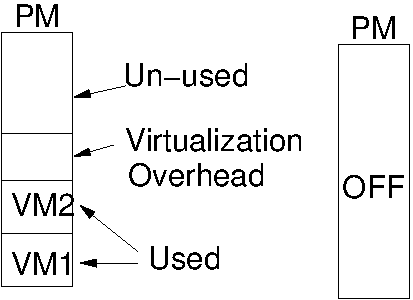
\includegraphics[scale=0.55]{presyn-figures/initially-consolidated.eps}} \hfill
%	%\subfloat[Initially VMs colocated on single PM]{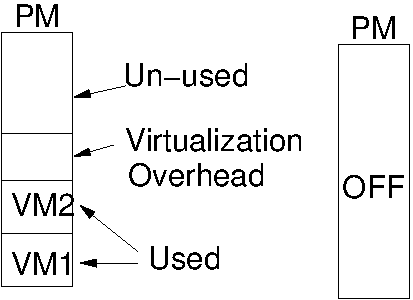
\includegraphics[scale=0.6]{presyn-figures/initially-consolidated.eps}} \hspace{0.6in}
%	%\subfloat[Slight load increase accommodated]{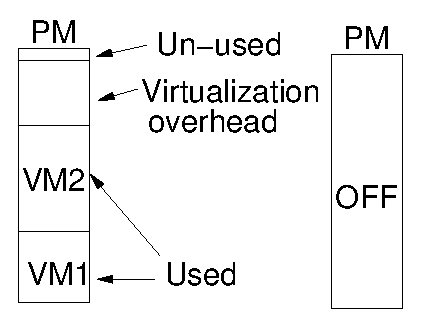
\includegraphics[scale=0.6]{presyn-figures/slight-load-increase.eps}} \\ \vspace{0.2in}
%	\subfloat[Slight load increase accommodated]{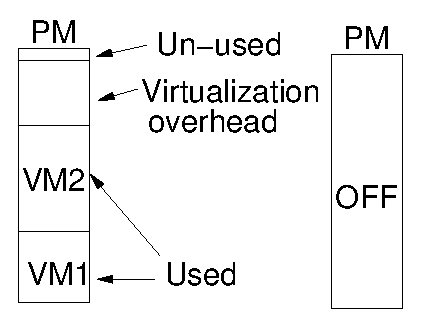
\includegraphics[scale=0.55]{presyn-figures/slight-load-increase.eps}} \hfill
%	\subfloat[Heavy load requires VM migration]{\includegraphics[scale=0.55]{presyn-figures/heavy-load-needs-migration.eps}} \hfill
%	\subfloat[Migrate back when load falls]{\includegraphics[scale=0.55]{presyn-figures/low-load-migrate-back.eps}}
%\caption{Server consolidation and migration for dynamic resource provisioning}
%\label{consolidation-migration}
%\end{center}
%\end{figure}

Virtualization enables dynamic resource allocation and quicker deployment
of services. Instead of installing new hardware for deploying a service,
virtualization allows transparent, on-demand deployment
on a few
processors in an existing multi-processor machine and avoids new machine
procurement delays. %~\cite{xen-art-of-virtualization}.
Virtualization allows accommodation of varying load-levels by
on-demand resource allocation %~\cite{xen-art-of-virtualization-revisited}
and also reduces application downtime. %~\cite{google-live-migration}.
Due to above benefits of virtualization,
many hosting centers have transitioned from providing 
Hardware as a Service (HaaS) to 
Infrastructure as a Service (IaaS) instead~\cite{ec2}.
The primary difference between HaaS and IaaS is that the
former involves use or leasing of physical
hardware/machine whereas the latter involves
leasing of virtual resources/machines.

Most web-based applications are multi-tiered and virtualization
offers the possibility of hosting each of these tiers (e.g., the 
web-server tier, the application logic tier and 
the database server) on separate virtual machines.
%elastically provisionable virtual machines. 
%Such differentiated hosting
%for various tiers is preferable 
%to hosting the entire %application as a monolithic entity 
%hosted on a single peak-provisioned %physical machine since 
%This enables independent and flexible resource management 
%of the different tiers. Additionally, due to
%elastic potential of resource allocation to virtual machines,
%differentiated hosting on virtual machines can help avoid resource
%wastage on under-utilized physical machines.
The major factors that affect the performance of a 
virtualized application are\textemdash{}available network capacity, disk access bandwidth
and virtualization overheads.
%When multi-tiered applications are instantiated in a virtual
%environment, the following major factors affect their 
%performance\textemdash{}available network capacity, disk access bandwidth
%and virtualization overheads. 
When multiple virtual machines (VMs) are placed on a single 
physical machine (PM),
they compete for various resources like CPU, memory, network and disk I/O
and interact in many conflicting ways. 
In any given virtualized environment, the physical resources available can 
be broadly categorized into the following:-

\paragraph{I. Resources allocated to the virtual machines.} 
Every virtual machine has access to a set of resources, similar
to those available on physical machines.
For example, virtual CPU, VM page cache, virtual disk, etc.
%are resources that are allocated to each virtual machine.
%These are
%usually statically allocated in today's datacenters~\cite{ec2}, 
%but can be better managed using dynamic provisioning 
%techniques~\cite{sandpiper}.

\paragraph{II. Resources in the virtualized host.} 
These are resources at the virtualized host to support and enable
virtualization.
For example, the hypervisor incurs CPU overheads
for virtualization. %~\cite{measuring-cpu-overhead}. 
The host's page cache is also used for buffering of physical I/O access,
on behalf of VMs.
\\
\\
In this thesis, we address two
important problems related to the management of both
these types of resources more efficiently, towards the overall goal
of optimizing the performance of virtualized applications and services.

\subsection*{Thesis contributions} 
\paragraph{1. Affinity-aware Modeling of CPU usage for Virtualized Applications.} 
This problem deals with managing the network 
usage of VMs and estimating CPU 
requirement on both the VM and its host PM.
Since different tiers of an application require mutual network
communication, \textit{colocation} of communicating VMs
on the same PM reduces physical network 
usage. \textit{Network affinity} is the presence of network
communication between a pair of VMs, and is 
\textit{intra-PM} when the VMs are colocated, and 
\textit{inter-PM} when they are dispersed onto different PMs.
Thus, the nature of network affinity is \textit{mutable} (i.e., changing
between inter-PM and intra-PM) upon VM migrations.
%We make the case that since there is significant change in CPU resource
%usage when the VMs are colocated versus when they are dispersed, it is
%essential to capture such changes, %via a model,
%for server consolidation and VM placement decisions.
%We define the presence of network traffic between a pair
%of VMs as their \textit{network affinity}, and state that the
%nature of this network traffic is \textit{mutable} based on
%whether the VMs are colocated or dispersed, i.e., network affinity
%can change between \textit{inter-PM} or \textit{intra-PM}
%upon VM migrations.
%can be \textit{inter-PM} or {intra-PM} based on whether the
%PMs are colocated on a single PM, or dispersed on different PMs. 
%In other words, the
%nature of the inter-VM network traffic can change between being
%intra-PM and inter-PM depending on whether the VMs are hosted
%on the same physical machine or on different physical machines.
%We explore the effect of the \textit{mutable}
%network traffic on CPU usage of colocated and dispersed VMs. More
%specifically, the question is

In our work, 
%we explore the difference in CPU utilization due
%to \textit{network affinity}, and propose models to
%estimate the changed CPU utilization.
%Specifically, 
we perform network benchmarking, which 
demonstrates effects of network affinity on CPU usage when VMs 
are colocated versus dispersed. Next, we develop VM \textit{pair-wise} models
that can estimate the ``colocated'' CPU usage, on being 
input their individual dispersed-case resource usages.
We also build similar models to estimate the ``dispersed'' CPU
usage based on the individual colocated-case resource usages.
For the ``colocation'' and ``dispersion'' models, we first 
built models that predicted the total (or absolute) CPU usage
upon migration\textemdash{}these CPU models use all resource (CPU, disk, mutable
and immutable network) usage profiles as their input. However, these models
had an error of around 4\%. So, next we built enhanced models
to predict only the difference (or differential) CPU usage\textemdash{}these
models use only the \textit{mutable} network traffic metrics as input,
and have maximum error within 2\%. Finally, we demonstrated the
application of \textit{pair-wise} models to predict for multi-VM
scenarios, with high accuracy.

\paragraph{2. Using Implicit Caching Hints for {D}isk I/O {R}eduction in Virtualized Environments.}
This problem deals with managing the cache
usage on a virtualized host to improve disk access performance 
of VMs.
Due to increased permeation of virtualization-based systems, there is a lot of
inherent content similarity in systems like email servers, web servers 
and file servers. 
%All this data resides on disk and is fetched by corresponding
%applications, as and when required. 
Harnessing content similarity can help 
avoid duplicate disk I/O requests that fetch the same content repeatedly.
In this work, we incorporate intelligent I/O redirection within the 
storage virtualization engine of the device to manage the underlying 
block-cache like a content-cache.

We build a disk read-access optimization called DRIVE, that
identifies content similarity across multiple blocks, and performs
hint-based read I/O redirection.
% than other systems.
A metadata store is maintained and implicit caching hints are collected 
based on the VM's disk accesses.
Using the hints, read I/O redirection is performed from within the VM's virtual
block device, to manipulate the entire
host-cache as a content-deduplicated cache.
Our trace-based evaluation using a custom simulator, reveals that
DRIVE achieves up to 20\% better cache-hit ratios and reduces
up to 80\% disk reads. It also achieves up to 
97\% content deduplication in the host-cache.

% \section{Thesis contributions}


%MERGED v2v-1 and v2v-2 into synopsis-arescue.tex, per advice from Puru.
\newpage
\section{Affinity-aware Modeling of CPU Usage for Virtualized Applications}
\label{sec:synopsis-arescue}
An important consideration for migration and consolidation related
decisions is the VM's resource requirement on the target host. 
%For mutually communicating VMs, 
%consolidation into a colocated set and migration to dispersed
%placements, can result in different CPU requirements.
VMs that mutually communicate are said to have \textit{network affinity}
and when VMs migrate, they may get colocated or dispersed w.r.t each 
other\textemdash{}resulting in different CPU overheads for network communication.
Network traffic between colocated VMs is considered \textit{intra-PM}, 
whereas between dispersed VMs is \textit{inter-PM}. Given a 
communicating VM pair, migration of one may cause change of network traffic
between them from \textit{inter-PM} to \textit{intra-PM},
or vice versa, depending on whether they get colocated or dispersed,
respectively\textemdash{}this is referred to as the \textit{mutable} nature 
of network affinity.
%due to \textit{mutable} nature of \textit{network affinity} between them.
In this work, we build
\emph{affinity-aware} models to predict expected CPU
requirements upon colocation or dispersion of VMs.
We make the following
contributions,
\begin{itemize}
		\singlespacing
%\vspace{-0.05in}
\vspace{-0.1in}
\item \emph{Event profiling} of intra-PM and inter-PM network 
	communication paths in Xen. % using \texttt{Xenoprof}~\cite{xenoprof}.
\item \emph{Benchmarking} of CPU usage
of VMs (Xen and KVM) for various workloads
in colocated and dispersed configurations.
\item Development of \emph{affinity-aware pair-wise} models to predict \textit{total}
	as well as \textit{differential} CPU usage, when a pair of VMs move between
	dispersed and colocated configurations.
%\item Apply above pair-wise models to \emph{multi-VM scenarios}, where
%a single migrating VM has more than one neighboring
%VMs with which it exhibits network-affinity, both on source \& target PMs.
\item Apply the pair-wise models to \textit{multi-VM scenarios} to predict CPU usage of a set of VMs.
\item \emph{Comprehensive evaluation} using synthetic workloads \& 
	benchmark applications, for pair-wise models as well as multi-VM scenarios.
\end{itemize}

%\subsection{Profiling study of Xen I/O virtualization}
%Using the tool \texttt{Xenoprof}~\cite{xenoprof}, we performed
%event monitoring for network transmission between a pair of Xen-based
%VMs in both colocated and dispersed scenarios.
%%~\cite{xen-internals, xen-networking, linux-networking}.
%%A common optimization in the colocated case is that packet 
%%check-summing is discarded, under the assumption that
%%memory copying (performed in colocated case) is quite reliable relative
%%to physical network transmission (corresponding to dispersed case).
%Colocated Xen-based VMs are
%connected to a layer 2 software bridge, so local network
%transmission is achieved via shared memory.
%However, network transmission between dispersed
%VMs is additionally
%DMA-copied\nomenclature{DMA:}{Direct Memory Access}\index{DMA}
%into the network interface
%card's (NIC\nomenclature{NIC:}{Network Interface Card}\index{NIC})
%buffer, and transmitted.
%Upon reception, packet is copied
%from NIC buffer into kernel buffer 
%and interrupt sent to host's driver domain (Dom0).
%The packet is subsequently inspected by Dom0
%and destination VM is notified. 
%Thus, end-to-end communication path is significantly longer in 
%dispersed case than colocated case.
%%These differences in CPU overheads were also observed empirically with
%both Xen and KVM environments, as presented next.

\subsection{Micro-benchmarking the effect of colocation on CPU Usage}
It is discussed in~\cite{virtual-putty}
that colocated provisioning can result in changes in
resource usage\textemdash{}however, empirical quantification is lacking.
We address the following questions,
(i) For communication between dispersed VMs, what is the 
change in CPU usage when VMs get colocated? 
(ii) For other network traffic and workloads, is colocated CPU usage a 
summation of dispersed usages?
%(iii) For pure CPU or disk workloads, is colocated CPU usage
%a summation of dispersed usages? 

%\begin{figure}[t]
%	\centering
%	\subfloat[Xen setup]{\includegraphics[scale=0.575]{jss-figures/benchmark}}
%	~~~~~~~~~~~~~~~~~~~~
%	\subfloat[KVM setup]{\includegraphics[scale=0.575]{jss-figures/kvmbenchmark}}
%	\caption{Setup for benchmarking, profiling and model evaluation.}
%	\label{fig:setup}
%\end{figure}

\begin{figure}
	\RawFloats
	\begin{minipage}{0.45\textwidth}
		\centering
		\includegraphics[scale=0.575]{jss-figures/benchmark}
		\caption{Setup for benchmarking, profiling and model evaluation.}
		\label{fig:setup}
	\end{minipage}
	\begin{minipage}{0.5\textwidth}
		\centering
		\includegraphics[scale=0.9]{arescue-figures/aff-benchmark/domU-cpu-vs-affine-rx-curve.eps}
		\includegraphics[scale=0.9]{arescue-figures/aff-benchmark/dom0-cpu-vs-affine-curve.eps}
		\caption{CPU utilization due to \textit{mutable} network traffic (in Xen setup).}
		\label{fig:cpuovhd-rxtx}
	\end{minipage}
\end{figure}	

%\vspace{-0.2in}
%\paragraph{Custom Micro-benchmarks:}
%We developed a multi-threaded load generation 
%tool, \texttt{LoadGen}, that generates
%CPU-intensive, network-intensive, disk-intensive and mixed workloads.
%Workloads are generated using a client-server setup,
%wherein a \textit{client} (the controller machine) remotely connects to
%the \textit{servers} (VMs), and invokes \texttt{LoadGen} command
%to generate desired workload.
%\vspace{-0.2in}
\paragraph{Setup:}
We developed a multi-threaded load generation 
tool, \texttt{LoadGen}, that generates
CPU-intensive, network-intensive, disk-intensive and mixed workloads.
We performed benchmarking for both Xen and KVM.
Fig.~\ref{fig:setup} shows the experimental setup that we
%The setup used for benchmarking with Xen virtualization technology
%is as shown in Fig.\ref{fig:setup}(a) wherein Dom0 is the privileged
%domain as described earlier in 
%Section~\ref{sec:litreviewchap-io-virtualization}.
%In case of KVM platform,
%there is no management domain since it
%does not follow the driver domain I/O model. Hence, the setup
%for KVM benchmarking is a slightly modified version, as
%depicted in Fig.~\ref{fig:setup}(b).
%As shown in the setup of Fig.~\ref{fig:setup}, 
used\textemdash{}two PMs host the VMs, and
each PM is connected via a Layer-2 Switch to an NFS server which hosts
the VMs' virtual disk images.
%disk images associated with the VMs. 
%Thus, all disk read/write
%operations are NFS-read/write operations which generate network traffic
%at the host. 
The Layer-2 Switch and all network links of the
machines operate at 100 Mbps.
The Controller uses scripts to automate
load generation and resource-usage measurements.
%Load generation is done using an automated script residing at the Controller,
%that invokes a custom application program (called \texttt{LoadGen})
%at each VM.
%Resource usages are measured using utilities like 
%\texttt{Xentop} (for Xen), %~\cite{xentop} (for Xen),
%\texttt{top} (for KVM),
%\texttt{sar}, and %~\cite{sar}, 
%\texttt{iptables}. %~\cite{iptables}.

%\begin{figure}%
%	\hspace{-0.3in}
%	\subfloat[DomU CPU utilization for Rx]{\includegraphics[scale=0.9]{arescue-figures/aff-benchmark/domU-cpu-vs-affine-rx-curve.eps}}
%%	\subfloat[DomU CPU utilization for Tx]{\includegraphics[scale=0.9]{arescue-figures/aff-benchmark/domU-cpu-vs-affine-tx-curve.eps}} \\
%	\centering
%	\subfloat[Dom0 CPU utilization for Rx/Tx]{\includegraphics[scale=0.9]{arescue-figures/aff-benchmark/dom0-cpu-vs-affine-curve.eps}}%
%	\caption{CPU utilization due to \textit{mutable} network traffic (in Xen setup).}
%	\label{fig:cpuovhd-rxtx}
%\end{figure}
%

\vspace{-0.4in}
\paragraph{Benchmarking results:}
%Hence we perform this benchmarking study of effect of
%network-affinity between two VMs\textemdash{}VM1
%and VM2 act as a Tx/Rx pair to transmit and receive data
%at different rates. 
%To study the implications of network-affinity
%between VMs, the experiment is conducted in both
%colocated and dispersed scenarios. The CPU utilization levels of both
%Dom0 and DomU are measured (refer Fig.~\ref{fig:cpuovhd-rxtx}).
Fig.~\ref{fig:cpuovhd-rxtx} plots DomU and Dom0 CPU utilization 
for varying network usage between a pair of VMs (i.e., \textit{mutable} 
traffic), in colocated
and dispersed scenarios. %\textemdash{}VM1 and VM2 form a Tx/Rx pair.
%As can be seen, with increase in network usage, benefits of VM colocation
%increase. 
At 90 Mbps, the colocated DomU utilization is 10\%,
which is almost half of the dispersed case.
%For the transmitting VM, the CPU utilization shows
%a decrease but very marginal.
%With close to 90 Mbps bandwidth utilization, the colocated
%CPU utilization is 10\%.
% This implies that there is definitely
% no increase in CPU utilization due to colocation of two 
% communicating VMs.
%Further, the absolute usage by Rx-network traffic is more
%than Tx-traffic for the same bandwidth\textemdash{}CPU utilization
%of 17\% and 9\% respectively, at 90 Mbps network bandwidth
%utilization.
%Fig.~\ref{fig:cpuovhd-rxtx}(b) shows corresponding Dom0 CPU usage.
Further, at 40 Mbps and 90 Mbps,
the difference in Dom0 CPU usage between
dispersed and colocated scenarios is 14\% and 25\%, respectively.
%dispersed (summation of utilization levels at both PMs in the
%dispersed scenario) and colocated (single
%Dom0 CPU) scenarios is 14\% and 25\%, respectively.

From our benchmarking, we concluded that differences in CPU usage across
colocated and dispersed placements occurs only for 
VMs that are mutually communicating, i.e., \textit{mutable} traffic. 
For workloads like CPU/disk workloads and 
\textit{immutable} traffic, different placements do not
affect CPU usage. 
Further, resource utilization and Dom0/DomU CPU utilization are linearly
related.

\subsection{Linear regression modeling for CPU requirement estimation}
%We run a set of benchmarks, also referred to as micro-benchmarks, in both
%scenarios\textemdash{}dispersed and colocated\textemdash{}which exercise the utilization
%levels of VMs along different
%axes\textemdash{}CPU, intra-PM and inter-PM network traffic, disk read and
%write operations.
\underline{Colocation and Dispersion models}:
We develop pair-wise CPU estimation models
that can predict total CPU requirement in target scenario
based on source scenario's resource usages. 
Specifically, using resource usage measurements of dispersed 
case, the ``colocation'' model predicts CPU utilization for 
colocated scenario, and based on resource usage in colocated case,
the ``dispersion'' model predicts for dispersed scenario.

Our benchmarking revealed that only the mutable network usage
causes changes in CPU requirement, upon a VM migration.
Hence, we build models to use \underline{two approaches of prediction}:-
(i)~Predict \textit{total} CPU requirement based on multiple 
resource usage profiles\textemdash{}CPU, disk and network,
(ii)~Predict \textit{differential} CPU requirement based only on
mutable network traffic metrics\textemdash{}later, take summation
of prediction with the source scenario's CPU usage to estimate
the total CPU requirement. Next, we briefly explain both the
approaches.

\subsection*{Approach 1: Prediction of total CPU requirement}

\paragraph{Intuition:} 
The total CPU requirement of a virtual machine accounts for all its 
activities, including usage of all other resources. Hence, this model
has all resource metrics as its
parameters: (i) $4$ metrics for mutable and
immutable transmit and receive network rates,
(ii) $3$ CPU metrics of \texttt{iowait}, \texttt{system}
and \texttt{user} CPU, and
(iii) $4$ metrics for disk read/write rates.
%blocks/second and bytes/second. 
%Since the correlation of all resource usages to CPU usage is linear, we employ
%linear regression methods to build the CPU estimation models.

\vspace{-0.2in}
\paragraph{Method:} We use multi-linear regression modeling, wherein
%Using values from the collected profiling data,
%the colocated CPU usage is represented as
%a linear function of the individually profiled resource metrics
%in the corresponding dispersed scenario (i.e. dispersed scenario
%stressed with the same workload),
%and similarly dispersed CPU usage is represented as a linear function of
%the colocated resource usage metrics.
the relation between estimated CPU and resource parameters is captured, 
as shown in Eqn. (\ref{mlr-eqn-1}).
\vspace{-0.2in}
\begin{equation}
\mbox{CPU}^{i}_{estimated} = C_{0} + C_{1} \times M^{i}_{1} + C_{2} \times M^{i}_{2} + ... + M^{i}_{m}
\label{mlr-eqn-1}
\end{equation}

\vspace{-0.2in}
\noindent where, $i$ is an iterator over each sample point,
$m$ is the number of parameters, $M^{i}_{j}$ is
the value of parameter $M_{j}$ collected in the sample point number 
$i$, and $\mbox{CPU}^{i}_{estimated}$ is the CPU usage
either after dispersion or after colocation of VMs.
%Thus, there are $11$ metrics in all to be considered.
% in Table~\ref{metrics-table}. 
%We build models for both DomU and Dom0 using the above multi-linear regression approach.
%Both the colocation and dispersion models for DomU have these $11$ parameters.
%The Dom0 \textit{colocation} model is built with metrics of both 
%DomUs\textemdash{}has $22$ parameters.
%The Dom0 \textit{dispersion} model
%depends on only one DomU's metrics at a time, and hence has only $11$
%parameters.
%For model building, we used 956 sample points in total\textemdash{}200 points 
%for CPU workload, 96 points for mutable network, 182 points
%for immutable network, 162 points for disk read, 158 points for disk write 
%and 158 mixed workloads.
To solve for the $m+1$ coefficients $C_{k}$, we use
Robustbase package, part of the R statistical computing environment.
%, for robust linear regression.
%The linear regression solver, takes as input $M^{i}_{j}$ values for the
%various workloads and outputs values of $C_{k}$ of best predict CPU utilization.
%The set of coefficients thus
%derived is the model that describes the relation between the $k$ parameters
%and the DomU and Dom0 colocated/dispersed CPU usage.

\subsection*{Approach 2: Prediction of differential CPU requirement}

\paragraph{Intuition:} The difference in CPU usage upon transition between
colocated and dispersed placements of a VM pair, depends only on the mutable
network affinity between them. Hence, we can predict only
the difference, and sum it with the original scenario's CPU usage, to
obtain the total CPU requirement.
The model parameters are bit-rates (in Kbps) and 
packet-rates (in packets per second) for both 
transmission (Tx) and reception (Rx), thus four parameters
in all. %: (i) Rx Kbps, (ii) Rx pkts/s, (iii) Tx Kbps, and (iv) Tx pkts/s. 
%Note that differential Dom0
%CPU is the difference in CPU usage between that incurred for the single (colocated) Dom0 and
%the summation of both (dispersed) Dom0.

\vspace{-0.2in}
\paragraph{Method:} 
Formally, Eqn. (\ref{cpu-diff-eqn}) captures the
general notion of change in CPU usage %($\Delta\mbox{CPU}$)
while transitioning between colocated and dispersed scenarios.
\vspace{-0.2in}
\begin{equation}
	% \hspace{-0.3in}
	\Delta\mbox{CPU} = \mbox{CPU}^{scenario1} - \mbox{CPU}^{scenario2}
	\label{cpu-diff-eqn}
\vspace{-0.2in}
\end{equation}
where, scenario$\{1|2\}$ = $\{colocated|dispersed\}$.
Each DomU and Dom0 model represented as
\vspace{-0.2in}
\begin{equation}
	\hspace{-0.3in} \Delta\mbox{CPU}_{est} = C_{0} + C_{1} \mbox{MutRx}_{Kbps} + C_{2} \mbox{MutRx}_{p/s} \\ 
	+ C_{3} \mbox{MutTx}_{Kbps}  + C_{4} \mbox{MutTx}_{p/s}
	\label{mlr-eqn}
\vspace{-0.2in}
\end{equation}
where, ``MutRx'' and ``MutTx'' stand for mutable network receive and transmit 
traffic, respectively. Once again, the Robustbase package %~\cite{robustbase}
is used to solve for the model coefficients.


\begin{figure}
\begin{floatrow}
\ffigbox{%
	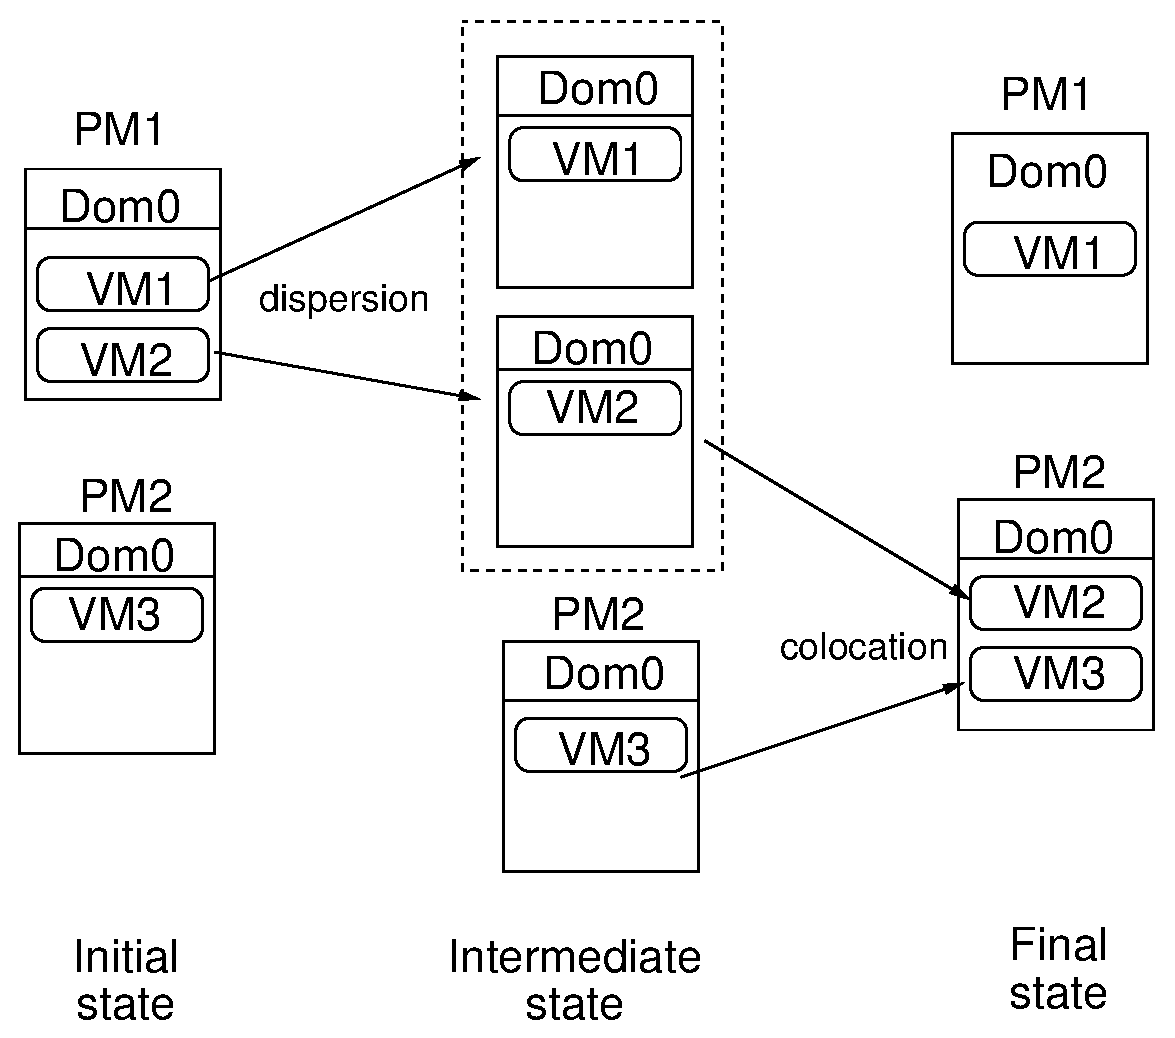
\includegraphics[scale=0.4]{jss-figures/new-forward-plus-rev.eps}
}{%
	\caption{Combined transition for $VM2$}
	\label{fig:forward-plus-reverse}
}
~~~
\vspace{-0.1in}
\small
\capbtabbox{%
	\begin{tabular}{|c|c|c|c|c|} \hline
		\textbf{Num} & \textbf{Max}  & \multicolumn{3}{|c|}{\textbf{Max error(\%CPU)}} \\  \cline{3-5}
	\textbf{of } & \textbf{n/w} & \textbf{DomU} &  \textbf{Dom0} & \textbf{Dom0} \\
    \textbf{clients} & \textbf{traffic} &  &  \textbf{colo} & \textbf{disp} \\ 
	\textbf{} & \textbf{(Mbps)} & \textbf{} &  \textbf{} & \textbf{} \\ \hline  %\cline{2-9}
  500 & 6.8 & 1.73 & 1.33 & 0.90 \\
	1000 & 13.4 & 1.50 & 0.98 & 0.82 \\
	1500 & 19.8 & 1.42 & 0.69 & 0.90 \\
	2000 & 26.4 & 0.90 & 1.08  & 1.21 \\
	2500 & 32.6 & 1.03 & 1.29 & 1.27 \\
	3000 & 39.4 & 1.36 & 1.50 & 1.54 \\ \hline
	\end{tabular}
}{%
	\caption{Model accuracy with varying load}
	\label{tab:xennumclients}
}
\end{floatrow}
\end{figure}

\subsection{Applying the pair-wise models to multi-VM scenarios}
%In a multi-VM scenario, any VM (say $VM_{x}$)
%may have multiple communicating neighbors, each belonging to
%exactly one of three sets, (i) \textit{affinity-at-source}
%(ii) \textit{affinity-at-target}, and (iii) \textit{affinity-at-other}.
%Migration of $VM_{x}$ will cause it to become dispersed from
%its \textit{affinity-at-source} set and colocated with its
%\textit{affinity-at-target} set\textemdash{}causing change in their CPU utilization.
In an example multi-VM scenario as shown in Fig.~\ref{fig:forward-plus-reverse},
migration of $VM2$ can cause it to be dispersed from $VM1$
and become colocated with $VM3$---we refer to this 
as a ``combined'' transition.
%Our aim is to predict the resource usage of all affected VMs and PMs.
%In Fig.~\ref{fig:forward-plus-reverse},
%CPU usages for $VM1$, $VM3$ and $PM1$ can be predicted by
%straight-forward application of \textit{colocation} and
%\textit{dispersion} models.
Here, CPU requirement estimation for $VM2$ and $PM2$ needs a
\underline{multi-phase prediction} methodology.
We need to first apply the \textit{dispersion model} to the
measured metrics corresponding to network-affinity level between $VM2$
and $VM1$, to get an intermediate estimate, and then apply the
\textit{colocation model} to the intermediate estimate
%This is an intermediate estimate and is used 
based upon network-affinity level
between $VM2$ and $VM3$ to get the final estimate.
%Intuitively,
%VMs in the \textit{affinity-at-other} set do not affect CPU
%requirement of the migrating $VM2$ because the nature of network-affinity
%between them stays the same (\textit{immutable}) both before and
%after migration.

\vspace{-0.1in}
\subsection{Summary of Experimental evaluation}
We generated CPU, disk, network and combinational workloads of
randomly picked levels to form our testing dataset.
Further, we used an application benchmark (RUBiS) to
perform testing\textemdash{}we generated different
levels of network traffic by using different number
of clients in each workload. Finally, we conducted
experiments with multi-VM scenarios wherein every
VM migration results in a different placement configuration,
and used the multi-phase prediction methodology 
to predict for every VM and PM.
Here, we present a list of main results. %subset of our results.

\begin{enumerate}
\singlespacing
	\item For both the approaches 1 and 2, we performed evaluation
with synthetic datasets and observed that Approach 1 (prediction 
of total CPU) had higher error of 4-5\% as compared to 
Approach 2 (prediction of differential CPU) error of 2\%.
	\item We conducted experiments with various number of clients
in RUBiS~\cite{rubis} and found maximum error
in each case to be within 2\% absolute CPU (refer Table~\ref{tab:xennumclients}). 
%This is tabulated in Table~\ref{tab:xennumclients}\textemdash{}maximum
%error is within 2\% absolute CPU.
	\item We created a 3-tier RUBiS setup and used the multi-phased
prediction methodology to predict the CPU usage of VMs and PMs 
across multiple transitions, and found maximum estimation error
within 2\% absolute CPU.
\end{enumerate}

%For further evaluation of our prediction models, we
%chose RUBiS~\cite{rubis}. It is 
%a two-tier application, consisting of a web tier and a database tier
%that communicate with each other for servicing user requests. Each tier
%is hosted in a separate VM.
%We generate repeatable RUBiS workloads in both dispersed and colocated cases,
%and compare average resource usages (predicted versus measured)
%over 30-second intervals. 
%The workload consisted of 800 clients
%generating site browsing load simultaneously, and requests being fired
%at determined times.
%We present a subset of our results here.

%\begin{figure}[h]
%	\centering
%	\includegraphics[scale=0.525]{jss-figures/rubis-3tier-layout.eps}
%	\caption{RUBiS 3-tier setup with proxy, webserver and database}
%	\label{fig:threetier}
%\end{figure}
%
%\vspace{-0.2in}
%\paragraph{Estimating CPU usage for ``combined'' transitions:}
%Fig.~\ref{fig:threetier} depicts our
%three-tier setup\textemdash{}we use Muffin proxy as the first tier of our test application.
%We consider a series of VM migration steps, each resulting in a different
%VM placement during a RUBiS run with 1000 clients.
%%and we apply \emph{colocation} and \emph{dispersion} models
%%appropriately to derive CPU usage prediction for each VM and PM. The series
%%of VM migration steps are 
%%(refer Fig.\ref{fig:migration-steps}):
%(a)~\textit{C0}: all 3 VMs on different PMs each (i.e. VM1 on PM1, VM2 on PM2, VM3 on PM3)
%(b)~\textit{C1}: VM2 migrates into PM1 and is colocated with VM1
%(c)~\textit{C2}: VM2 migrates into PM3 and is colocated with VM2
%(d)~\textit{C3}: VM2 migrates into PM2, same as initial configuration.
%
%The maximum error in prediction of Dom0 CPU for each step is listed in
%Table \ref{tab:vm-steps-error}, and is within 2\% for all transitions.
%The entry NA in any
%particular column implies that prediction is not performed for that
%PM during that step. This could be due to one of two reasons: (i) Due to
%the VM migration step, the PM has become idle, or (ii) During the
%VM migration step, the PM is not the source or destination of
%migration.
%
%\begin{table}[t]
%	\begin{tabular}{ |c|c|c|c|} \hline
%		\textbf{Transition} & \multicolumn{3}{|c|}{\textbf{Maximum error in Dom0 prediction}} \\
%														   % & \multicolumn{3}{|c|}{\textbf{in Dom0 prediction}} \\
%		 & \multicolumn{3}{|c|}{\textbf{(\% absolute CPU)}} \\ \cline{2-4}
%		 & \textbf{PM1} & \textbf{PM2}  & \textbf{PM3} \\ \hline  %\cline{2-9}
%		\textit{C0}$\rightarrow$\textit{C1} & 0.75 & NA & NA \\
%		\textit{C1}$\rightarrow$\textit{C2} & 1.99 & NA & 0.85 \\
%		\textit{C2}$\rightarrow$\textit{C3} & NA & 0.51 & 0.43  \\ \hline
%	\end{tabular}
%}{%
%	\caption{Dom0 CPU prediction error across different placement configurations.}
%	\label{tab:vm-steps-error}
%\end{table}
%

\vspace{-0.2in}
\subsection{Conclusions}
In this work, we performed network benchmarking, to 
quantify the effects of network affinity on CPU usage when VMs
are colocated versus dispersed. 
%We built affinity-aware CPU estimation models for a pair of communicating
%VMs, which is generic and application-agnostic. 
Next, we developed VM \textit{pair-wise} models
that can estimate ``colocated'' CPU usage, on being
input their individual dispersed-case resource usages,
and to estimate ``dispersed'' CPU
usage based on colocated-case resource usages, using two approaches.
Experiments revealed that Approach 2 provides better estimates
with maximum error less than 2\%.
%For the ``colocation'' and ``dispersion'' models, we first
%built models that predicted the total CPU usage
%upon migration\textemdash{}these CPU models use all resource (CPU, disk, mutable
%and immutable network) usage profiles as their input. However, these models
%had an error of around 4\%. So, next we built enhanced models
%to predict only the differential CPU usage\textemdash{}these
%models use only the \textit{mutable} network traffic metrics as input,
%and have maximum error within 2\%. 
Finally, we demonstrated the
application of \textit{pair-wise} models to predict for multi-VM
scenarios, with high accuracy.
%We tried two approaches
%of modeling and found that predicting differential CPU usage provided
%better accuracy\textemdash{}with maximum error within 2\% absolute CPU usage.
%We also demonstrated that simple 
%This proves that CPU usage prediction models built
%on the scale of two VMs can be used for prediction in multi-VM
%scenarios as well.


%\newpage
%\section{Affinity-aware Modeling of CPU Usage for Virtualized Applications}
%\label{sec:synopsis-v2v-1}
%\input{synopsis-v2v-1}
%\newpage
%\section{Enhanced Affinity-aware Modeling of CPU usage for Virtualized Applications} 
%\label{sec:synopsis-v2v-2}
%\input{synopsis-v2v-2}

\newpage
\section{DRIVE: Using Implicit Caching Hints to Achieve \underline{D}isk I/O \underline{R}eduction \underline{i}n \underline{V}irtualized \underline{E}nvironments} 
\label{sec:synopsis-drive}
Content similarity within a single VM image is called intra-VM similarity and across multiple
VMs is referred to as inter-VM similarity. A study of content similarity amongst 525 VM images
from a production environment~\cite{similarity}
reported 30\% blocks repeating at least twice and 12\% blocks
repeating 5 times. A study in \cite{intra-higherthan-inter} 
reported that up to 90\% of total similarity observed among VM
disk content is intra-VM, rather than inter-VM. 
The work in \cite{iodedup} 
studied the degree of content
similarity in application workloads (web, mail and file system) hosted in VMs, and reported that
there are multiple blocks having identical content within each application workload.

A VM's virtual disk is present on the host's storage, which may be a local disk 
or a network-attached remote disk. 
Disk access times are in the order of a few 
milliseconds~\cite{google, data-domain}, whereas cache
access timings are orders of magnitudes lower~\cite{pagecache, satori}. 
Hence, improving caching effectiveness can
help improve storage access performance and overall application performance. However, due to
content similarity across blocks, host cache effectiveness is limited by two factors: (i) duplicate
I/O problem\textemdash{}multiple blocks containing same content being fetched from disk, 
and (ii) duplicate content problem\textemdash{}multiple blocks in cache have same content. 
Both problems can be
addressed by maintaining content similarity metadata by actively tracking insertion and eviction
of blocks in page cache, however this would require invasive changes in the host kernel.
We develop a read I/O redirection technique positioned within the VM's virtual block device,
such that both problems are addressed. If a block of content is present in the host's page-cache,
it need not get fetched from disk. This, in turn, ensures that multiple blocks with same content
are (almost) never stored into the host's page-cache, i.e., a content-deduplicated page-cache is
achieved. Thus, we reduce disk I/O without actively tracking page-cache state, as well as without
maintaining any explicit content cache. The \textbf{contributions} of this work are,
\begin{enumerate}
	\singlespacing
\item Simulation-based analysis of existing system \cite{iodedup} to show that it is inefficient.
\item Design and implementation of the DRIVE system that tackles both the duplicate content
and duplicate I/O problems,
\item Trace-based evaluation of DRIVE with prototype implementation in a custom simulator.
\end{enumerate}

\begin{table}
%\vspace{0.1in}
\caption{Summary statistics of traces used for evaluation}
\label{tab:stat-summary}
\centering
%\noindent\makebox[\textwidth]{% 
\begin{tabular}{|l|c|c|c|c|c|c|c|} \hline
	\textbf{Trace} & \textbf{Num of} & \textbf{Num of} & \textbf{Max} & \textbf{Max} & \textbf{\%blks} & \textbf{\%content} & \textbf{Write} \\
	 \textbf{Name} & \textbf{read} & \textbf{write} & \textbf{share} & \textbf{occur} & \textbf{having} & \textbf{occuring} & \textbf{intensivity} \\
			   \textbf{} & \textbf{requests} & \textbf{requests} & \textbf{factor} & \textbf{factor} & \textbf{2 copies} & \textbf{twice} & \textbf{factor}  \\ \hline
	\textit{homes} & 4,052,176 & 17,110,222 & 5904 & 5905 & 5 & 10 & 4.2 \\ \hline
	 \textit{mail} & 2,375,409 & 18,007,471 & 57015 & 57015 & 5 & 6 & 7.6 \\ \hline
	\textit{webvm} & 3,116,456 & 11,177,702 & 124 & 125 & 35 & 45 & 3.6 \\ \hline
\end{tabular}
%}
%\vspace{-0.3in}
\end{table}

\begin{figure}
	\RawFloats
	\begin{minipage}{0.45\textwidth}
	\includegraphics[scale=0.55]{confided-figures/main/sys-arch-iodedup-host.pdf}
	\vspace{-0.25in}
	\caption{System Architecture of IODEDUP}
	\label{fig:iodedup-arch}
	%\vspace{-0.2in}
	\end{minipage}
	\hfill
	\begin{minipage}{0.47\textwidth}
	    \includegraphics[scale=0.60]{confided-figures/sweetspot-512MB/sweetspot-512MB.pdf}
			\vspace{-0.5in}
			\caption{Hit ratios in IODEDUP upon \textit{webvm}; total cache size is 512 MB.}
			\vspace{-0.05in}
			%, and content-cache size as the specified \% of the total.}
			\label{fig:sweetspot-512MB}
		\end{minipage}
\end{figure}
\vspace{-0.2in}

%\vspace{-0.2in}
\subsection{Analysis of existing I/O deduplication technique: IODEDUP}
Harnessing content similarity to avoid duplicate disk I/O requests is called I/O deduplication.
The work in \cite{iodedup} 
builds metadata regarding block content similarity, and maintains a content-
cache\textemdash{}retains a single copy of each content. Fig.~\ref{fig:iodedup-arch} 
shows I/O Deduplication (henceforth IODEDUP) system architecture. 
When read requests encounter a block-cache miss, they are 
intercepted by IODEDUP system and serviced from content-cache, if possible\textemdash{}thus avoiding 
duplicate content fetches from disk. However, since only a fraction of total space can be reserved
as content-cache, the \underline{duplicate content problem persists}. 
Secondly, since the content-cache
partakes from total memory space available, 
\underline{optimally sizing the content-cache is essential}
because content-cache benefits may be application or request-mix specific.

\vspace{-0.2in}
\paragraph{Simulation setup:} We built a custom simulator, \texttt{SimReplay}, 
with prototype implementations
of Vanilla and IODEDUP systems. In Vanilla system, a read request's block number is first
looked up into block-cache. If not found in cache, the block is fetched
from disk. In IODEDUP system, the disk fetch path due to block-cache miss is intercepted 
and metadata is used to lookup the block in content-cache. A content-cache hit averts
the disk fetch, however, a miss necessitates disk fetch and metadata update. For exploration of
IODEDUP system's effectiveness, we chose six content-cache size settings as 10\%, 20\%, 30\%,
50\%, 70\% and 90\% of the total memory size, and remaining as the block-cache size.

\vspace{-0.2in}
\paragraph{Traces for simulation:} We borrow traces provided via \cite{iodedup} 
which are over 21 days from three
production systems: (i) webvm--from virtualized web-servers hosting webmail proxy and course
management system, (ii) mail--email server traces, and (iii) homes--file server traces. 
Table \ref{tab:stat-summary}
presents a summary of the traces. %, shows that webvm workload is likely to benefit most from
%deduplication techniques, due to higher percentage of content sharing and occurrence.

\vspace{-0.2in}
\paragraph{Analysis results:} Fig.~\ref{fig:sweetspot-512MB} 
shows cache-hit ratios for webvm trace for read-only, write-only and
read-write replays. IODEDUP has different optimal content-cache sizes for different 
cases\textemdash{}90\% for read-only, 10\% for write-only, and 10\% for read/write. 
Further, for read-write trace, performance of IODEDUP worsens compared to Vanilla, 
as content-cache size increases. Hence,
we consider 10\% as optimal content-cache size for further evaluation.

\begin{figure}
	\RawFloats
	\begin{minipage}{0.4\textwidth}
    \centering
    \includegraphics[scale=0.5]{confided-figures/main/deduped-block.pdf}
%    \vspace{-0.15in}
%    \caption{Semantics of metadata store in DRIVE system: \textit{each block points to a unique deduplicated block, and each deduplicated block reverse maps to multiple actual blocks}}
	\caption{Metadata store semantics: \textit{each block points to a unique deduplicated block, and each deduplicated block reverse maps to multiple actual blocks}}
    \label{fig:deduped-block}
%    \vspace{-0.2in}
	\end{minipage}
	\hfill
	\begin{minipage}{0.55\textwidth}
    \centering
    \includegraphics[scale=0.5]{confided-figures/main/dedup-working-readflowcomp.pdf}
    \caption{Flow path(s) for read in DRIVE: \textit{P is requested block, Q is corresponding ``leader'' block.}}
    \label{fig:confided-working(b)}
%     \vspace{-0.25in}
	\end{minipage}
\end{figure}
\vspace{-0.2in}


\subsection{DRIVE system requirements and design}
We build an I/O redirection system positioned above the block-cache which uses implicit caching
hints to perform the redirection.
%\vspace{-0.2in}
%\paragraph{System requirements.} 
The \textbf{system requirements} of an efficient I/O reduction system:
\begin{enumerate}
	\singlespacing
	\small
\item Fingerprinting mechanism to identify content similarity across different blocks.
%\item Data-structures to store metadata for similar blocks.
\item Maintaining implicit caching hints within metadata to aid future I/O redirection.
\item Interception of block read request path for metadata lookup and I/O redirection, if present.
\item Interception of block read return path for metdata update, if not previously present.
\item Interception of block write request path for metadata invalidation.
\end{enumerate}

\vspace{-0.2in}
\paragraph{System Design.} 
The DRIVE system has three main components: (i) \textit{Metadata maintenance},
(ii) \textit{Maintaining implicit hints regarding host-cache state}, 
(iii) \textit{Hint-based read I/O redirection}.

\textbf{(i)~Metadata maintenance}: 
%Metadata is updated for every new block of content , encountered
%in two ways: (i) every block of data written to cache, %for later flushing to disk, 
%(ii) every read
%request for an as yet unseen block fetched from disk. 
For read requests,
we compare content fingerprints to determine whether it is ``new'' or ``duplicate'', and
update metadata accordingly. For write requests, we invalidate existing mappings for those
blocks, so that stale metadata is not used for the next read request redirection.
The semantics of metadata store is as illustrated 
in Fig.~\ref{fig:deduped-block}.

\textbf{(ii)~Maintaining hints regarding host-cache state}: 
To avoid invasive tracking of host-cache (i.e., by trapping and intercepting each 
insertion and eviction within cache), we use \textit{implicit hints}
for redirection instead. When a read request is serviced, the corresponding physical block is in
host-cache, and if found to be identical to any previously requested block, we record the current
block ID as ``leader'', for that content. The recording as leader is done to aid redirection of future
I/O requests that request the same content, and is a hint regarding the state of host-cache.
%, and do not
%guarantee a cache-hit. However, hints offer a good chance of encountering a cache-hit to fetch
%the same content, without explicitly tracking host-cache.

\begin{figure}
    \RawFloats
    \begin{minipage}{0.45\textwidth}
    \centering
    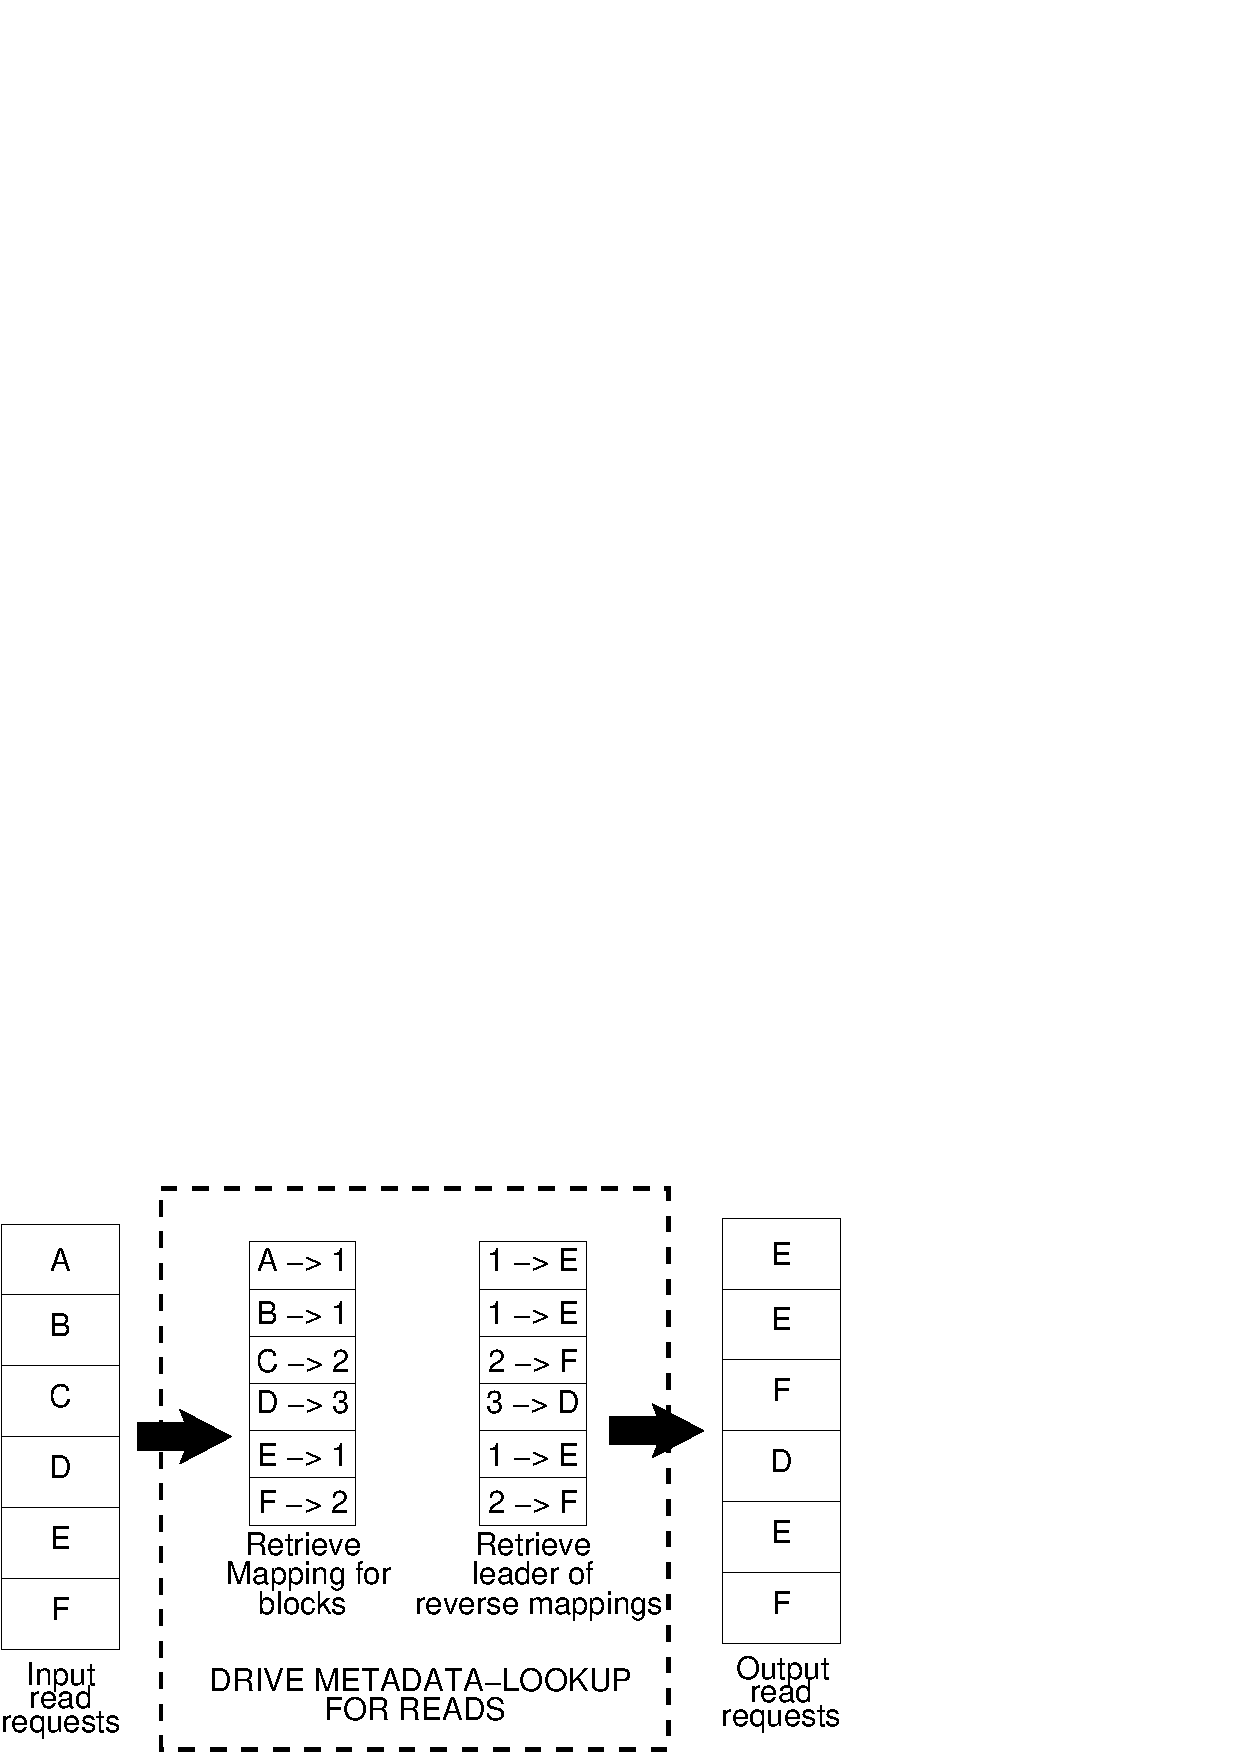
\includegraphics[scale=0.5]{confided-figures/main/dedup-working-reads.pdf}
%    \vspace{-0.125in}
    \caption{Read request redirection in DRIVE}
    \label{fig:confided-working(a)}
%    \vspace{-0.15in}
	\end{minipage}
	~~~~~
    \begin{minipage}{0.55\textwidth}
    \centering
	\includegraphics[scale=0.8]{confided-figures/contentdedup-factor/contentdedupfactor.pdf}
	\vspace{-0.6in}
	\caption{Host cache effectiveness upon \textit{webvm} trace.}
	\label{fig:contentdedup-factor-timeseries}
%    \vspace{-0.2in}
	\end{minipage}
\end{figure}

\textbf{(iii)~Read I/O redirection using implicit hints}: 
Before a read request hits the host-cache, the DRIVE
system intercepts it and looks up metadata to check for a recorded leader. If present, original
block ID in request is replaced with the leader block ID. Fig.~\ref{fig:confided-working(b)} 
depicts the multiple flows in
the read path, wherein an incoming request for block P is looked up in metadata store and if
successful, redirected to block Q.

\underline{Overall operation}: Fig.~\ref{fig:confided-working(a)} 
illustrates via an example. Suppose blocks A, B and E have identical
content (mapped to deduplicated ID 1) and E is appointed their leader since it was fetched the
latest. Whenever next, read requests for A, B or E are received, request is redirected to read
block E. Note that, blocks A, B and C will be in cache the first time they are fetched but once
they get evicted, they will never enter cache again, unless writes are done to them. This implies
that the cache is operated in an almost fully content-deduplicated fashion, hence improving its
effectiveness in reducing the number of disk reads.

%\vspace{-0.2in}
%%\paragraph{System implementation.} Fig.~\ref{fig:metadata-structure} 
%shows summary of metadata store 
%implementation\footnote{The CPU and memory overhead analysis is present in the thesis}. It con
%sists of an array containing entries for every block, a hash-table containing entries for every
%deduplicated block, and an array of pointers indexed by deduplicated block ID, pointing to the
%corresponding entry in hash-table. Each hash-table entry corresponds to one deduplicated block,
%has a list of reverse mapped block IDs, as well as content fingerprint. The fingerprint technique,
%used for duplicate content identification, can be any collision-resistant hash function. For leader
%identification, the list of reverse mappings is a Last-in-First-Out (LIFO) list. If the leader block
%content changes due to a write request, it is removed from the list of reverse mappings and the
%next most recently fetched block ID becomes new leader.

%\begin{figure}[t]
%%   \centering
%    \subfloat[Cache-hit performance]{\includegraphics[scale=0.55]{confided-figures/cache-hit-rate/reads-writes/eval-reads-n-writes.pdf}} \hfill
%    \subfloat[Disk read reduction]{\includegraphics[scale=0.55]{confided-figures/disk-fetches-averted/reads-writes/readsaverted-reads-n-writes.pdf}}
%    \caption{Comparison based on \textit{measured metrics} for read/write traces}
%    \label{fig:eval-read-write-perf-a}
%	\vspace{-0.1in}
%\end{figure}

%\begin{figure}
%    \RawFloats
%    \begin{minipage}{0.4\textwidth}
%    \centering
%    \includegraphics[scale=0.49]{confided-figures/read-response-distrib/reads-writes/read-response-distrib-reads-n-writes.pdf}
%    \caption{Classification of read responses in Vanilla Vs IODEDUP Vs DRIVE for \textit{homes}, \textit{mail} and \textit{webvm}.}
%    \label{fig:eval-read-write-perf-c}
%	\end{minipage}
%	\hfill
%    \begin{minipage}{0.59\textwidth}
%	\centering
%	%\vspace{-0.1in}
%	\end{minipage}
%\end{figure}
%\vspace{-0.2in}

\subsection{Summary of experimental evaluation}
For evaluation, we extend our simulator, and replay same traces as before. 
%Every record in the
%trace file contains:- (i) block number to be read or written, and (ii) MD5 hash of content. 
For every trace replay, measures like cache hits, cache misses, and disk fetches are recorded.
We performed evaluation for individual (single-VM) 
workloads, as well as simultaneous (multi-VM) workloads. 
Here, we present a summary list of main results.

\begin{enumerate}
	\item Our evaluation shows that with webvm workload,
		DRIVE has \underline{higher cache-hit ratios} than both 
		Vanilla and IODEDUP systems, 10\% and 20\% better, respectively.
		Moreover, DRIVE has higher number of ``disk reads reduced'', with nearly
		85\% improvement over Vanilla, and a 2.8$\times$ improvement over IODEDUP.
	\item A \underline{classification of read request responses} into compulsory misses, capacity misses
		and cache hits, for each trace, showed that \textit{webvm} trace contained a
		lot of capacity misses in the Vanilla system, and DRIVE succeeds in reducing 
		them to 5\% of the Vanilla system.
	\item We define \underline{content deduplication factor} as the ratio of
number of unique content blocks to total number of blocks in cache. Thus, higher the content
deduplication factor, better is cache efficiency. Fig.~\ref{fig:contentdedup-factor-timeseries} 
shows the variation in content deduplication factor, as each request of the webvm trace is replayed. We see that DRIVE system achieves
significantly higher content deduplication than both Vanilla and IODEDUP\textemdash{}a content 
deduplication factor of up to 97\%.
	\item To perform \underline{evaluation of multi-VM workloads} executed on a 
		virtualized host, we aggregated the \textit{homes} and \textit{webvm} 
		traces in timestamp order, and replayed it.
The metrics tabulated in Table~\ref{tab:aggregate-hw} 
show that although the cache-hit ratios are comparable in all
three schemes, DRIVE system averts 18\% disk reads as compared to 1.6\% of Vanilla and 4.3\%
of IODEDUP. Fig.~\ref{fig:aggregate-hw-time-series} 
plots the read response throughput per hour, assuming continuous replay
of requests. We can see that DRIVE produces more number of responses per hour in the 4th,
5th, 6th hours and so on, hence resulting in earlier completion than Vanilla or IODEDUP.
\end{enumerate}

%content deduplication of page cache can not be achieved because of compulsory misses incurred
%during cache-warmup, as well as cache dirtying by write requests. However, 
%DRIVE attains a high content deduplication factor of up to 97\%.

\begin{figure}
\begin{floatrow}
\ffigbox{%
\includegraphics[scale=0.7]{confided-figures/aggregate-hw-replay/reads-writes/timeseriesperf-hour.pdf}
}{%
\caption{Read throughput for aggregate trace}
\vspace{-0.55in}
\label{fig:aggregate-hw-time-series}
}
~~~
\vspace{-0.1in}
\capbtabbox{%
\begin{tabular}{|c|c|c|} \hline
\textbf{Scheme} & \textbf{Hit} & \textbf{Reads} \\
\textbf{} & \textbf{rate(\%)} & \textbf{saved(\%)} \\ \hline
%\textbf{} & \textbf{} & \textbf{} & \textbf{latency} \\ \hline
Vanilla & 61.2 & 1.6 \\ \hline
DRIVE & 67.6 & 18.5 \\ \hline
IODEDUP & 62.4 & 4.3 \\ \hline
\end{tabular}
}{%
	\caption{Aggregate replay performance}
	\label{tab:aggregate-hw}
}
\end{floatrow}
\end{figure}

\vspace{-0.05in}
\subsection{Conclusions}
In this section,
we considered the problem of improving disk access performance by improving host
cache efficiency. Typically, caches are referenced by block number, and can not recognize con-
tent similarity across multiple blocks. 
%Hence, the system ends up storing multiple copies of same content into cache. 
Elimination of duplicate read I/O requests is referred to as I/O Deduplication.
Existing work (IODEDUP) uses a split-cache approach~\cite{iodedup}, 
with a part of block-cache reserved as a content-cache. 
We demonstrated that a split-cache approach is inefficient, and presented
the DRIVE system which performs I/O redirection to implicitly manipulate the whole underlying
cache as a content-deduplicated cache. Only the VM's own disk access history is introspected
to obtain implicit hints regarding host cache state, to be used for read I/O redirection.

We performed comparative trace-based evaluation in a custom simulator. The evaluations
showed that, the DRIVE system achieves a high content deduplication factor of up to 97\%. This
is the key reason for better performance, with up to 20\% higher cache-hit ratios, and up to 85\%
higher number of disk reads reduced than the Vanilla system.


%\subsection{Discussion and future work}
%\paragraph{Further evaluation.} Based on an extensive literature survey of 100+ publications and 350+
%datasets, we concluded that there are no realistic benchmarking tools or trace generation frame-
%works for evaluation of I/O deduplication techniques. Thus, we need to either collect multiple
%production workload traces, or create frameworks that can synthesize realistic I/O traces having
%content representation, for further research in this area.
%\paragraph{Applicability to other storage systems.} The IODEDUP system uses ARC policy to boost
%up its content-cache hit ratio by 3-4X~\cite{}. 
%DRIVE performance could also get a boost if the
%host-cache policy is changed to ARC. Although this is unlikely in a standard Linux host, ARC
%caches are present in IBM's DS6000/DS8000 storage controllers, so adoption of DRIVE may
%help increase their cache performance.





%\newpage
%\section{The Case for I/O Deduplication Benchmarks}
%\label{sec:synopsis-architecting}
%In general, higher the amount of
duplicate content in the traces, higher the effectiveness of any
I/O deduplication technique.
However, as our evaluation showed,
even though \textit{webvm} trace had high levels
of duplicate content,
%and was an ideal candidate to benefit from I/O deduplication techniques, 
the deduplication benefits achievable for it was poor in IODEDUP system 
and great within the DRIVE system. This indicates that not just
the degree of duplicate content, but possibly other characteristics
also contribute to such varied performance.
To evaluate the DRIVE system further, we had the following options:-
\begin{enumerate}
		\singlespacing
    \item Build our own tracing toolkit (\texttt{preadwritedump}) to capture more traces.
    \item Deploy above toolkit on production servers to capture real-world traces
    \item Deploy above toolkit to capture synthetic benchmark traces
    \item Perform survey to find real-world datasets for I/O deduplication evaluation. 
    \item If public datasets available, use them for further testing of DRIVE system
    \item Extensively characterize the available traces to learn which particular properties of the \textit{webvm} trace contributed to its enhanced performance in the DRIVE system
    \item If public datasets not available, build a case for synthetic I/O deduplication benchmarks
\end{enumerate}

\subsection{Building trace collection toolkit}
%Of the above alternatives, we started off with building our own tracing
%toolkit with a view to deploying it on production servers within our
%department. 
We designed and implemented the I/O tracing toolkit 
called \texttt{preadwritedump}, however,
we were unable to obtain requisite permission from the systems
administrators to deploy it on the departmental servers. Thus, although
we could not fully utilize the developed tool, we believe that it would
be helpful for future tracing efforts.

\subsection{Use synthetic benchmarks}
%The next alternative was to execute synthetic workloads and capture 
%corresponding traces. However,
The challenge here is to execute synthetic workloads that are ``realistic''.
Many public storage and I/O benchmarks exist, however, their
focus is only on the number of I/Os per second, and not on the I/O content.
%Hence, these benchmarks tend to generate ``realistic'' workload levels 
%(i.e., number of IO
%operations per second) while paying scant attention to
%whether the content being generated as part of the read and write
%operations are also realistic or not.
For example, RUBiS is an application benchmark mimicking
an e-commerce website but most of its content pages are dummy pages (eg.
containing repetitive ``item descriptions'' or ``comments''). 
This duplicate content is accidental, and is not
representative of real e-commerce applications' content.
%Alternatively, the duplicate data created in HiBench benchmark is for
%the express purpose of storage availability in bigdata or MapReduce 
%environments,
%hence deduplicating such blocks on storage is counter-productive.

\subsection{Survey of datasets and benchmarks in literature}
\begin{figure*}
    \centering
    \subfloat[Conference-name tag cloud]{\includegraphics[scale=0.2]{presyn-figures/conference-names-wordle.jpg}} \hfill
    \subfloat[Year-of-publication tag cloud]{\includegraphics[scale=0.2]{presyn-figures/year-of-publication-wordle.jpg}}
    \\
    \caption{Representation of the conferences and the years of publication covered in our survey}
    \label{fig:tag-clouds}
\end{figure*}

%Due to above unsuccessful attempts at generating synthetic workload traces
%for evaluation of DRIVE, we once again turned towards datasets in literature
%and performed an extensive survey to determine whether any
%relevant useful datasets are available online.
We surveyed the datasets used in over
100 publications amounting to over 350 datasets\textemdash{}the tag clouds
in Fig.~\ref{fig:tag-clouds}(a) and (b) represent our survey coverage.
To begin with, we classified the dataset surveyed into
two sets: 
(i)~\textit{Proprietary datasets}\textemdash{}these are mentioned in various
papers but are not publicly available,
(ii)~\textit{Public datasets}\textemdash{}these are publicly available
online.
%and can be used by any researcher with an Internet connection.
%For example,
%the research groups from NetApp, IBM, etc use trace datasets that are
%internally available to them, but are not published online.
%For each of these datasets, we need to distinguish the dataset further based 
%on their context as follows:-
%(i)~Storage I/O traces with content representation,
%(ii)~Storage I/O traces without content representation,
%(iii)~Storage metadata with content representation, or
%(iv)~Storage metadata without content representation.
%The first item in the above list is the kind of trace we are looking for,
%i.e. I/O activity traces with content representation. However, we found
%that almost all of the public datasets available online fall in one of
%the other three categories listed above.

\paragraph{Proprietary datasets.}
Most datasets cited in literature are rarely hosted
publicly~\cite{generating-datasets}, hence unavailable to
other researchers for comparative analysis. 
We present a brief categorization.
%(In the thesis, 
%we cite the works which have used each category of dataset, although we
%omit that discussion here for the sake of brevity).

\begin{enumerate}
	\singlespacing
 \item \textit{Homes:} Shared-storage hosted home directories of
 employees or students or researchers.
 %~\cite{primary-data-dedup, backup-workloads-characterization, 
%datadomain, cifs-study, redundancy-alternatives}.
 \item \textit{CollaborationShares:} Shared-storage hosted directories
 among researchers or collaborators.
% created by one user and read/updated by many.
 %~\cite{content-sampling, idedup, cifs-study, redundancy-alternatives}.
 \item \textit{WebServer:} Webserver and Web-search workloads.
 %~\cite{storagecharacterization, filesystem-workloads, 
 %content-sampling, my-cache-or-yours, filesize-distrib-cause, 
 %web-cable-modem, scaling-phenomena, web-client-access-patterns}.
 \item \textit{SoftwareDeployment:} VM images, softwares, binaries 
	 for deployment by users.
 %~\cite{similarity, iodedup, redundancy-alternatives}.
 \item \textit{VM-Dataset:} VM images with
 different operating systems, applications and libraries.
 %~\cite{similarity, dedup-effectiveness}.
 \item \textit{VM-Backup:} VMs fully or partially backed up regularly, 
	 causing significant redundancies.
 \item \textit{DatabaseBackup:} Database backup storage and workloads.
 %~\cite{ddelta, hybrid-dedup, 
 %backup-workloads-characterization, ventana}.
 \end{enumerate}


\paragraph{Public dataset repositories.} 
%Below we provide a listing of those online trace repositories,
%which contain huge number of traces (i.e. multiple trace sets, not just one)
%and are available to the researchers for development and analysis of network
%and storage systems.
\begin{enumerate}
		\singlespacing
    \item \textbf{SNIA IOTTA Repository}: Provides storage-related I/O traces, tools and analysis.
    \item \textbf{HP Labs Repository}: Provides filesystem and application traces, albeit outdated.
    \item \textbf{UMass Trace Repository}: Provides network, storage, and other traces.
    \item \textbf{Internet Traffic Archive}: Provides access to traces of Internet network traffic.
    \item \textbf{VMware image repository}: Provides VMware images with various Linux distributions installed like CentOS, Debian, Fedora, FreeBSD and OpenSUSE.
    %\item FSL labs repository
    %\item LiveDFS repo?
\end{enumerate}

\paragraph{Public individual datasets.}
\begin{enumerate}
		\singlespacing
    \item \textbf{I/O deduplication traces}: Traces provided via~\cite{iodedup}, which we used in our evaluation.
    \item \textbf{Plan 9 traces}: Snapshots of Plan 9 filesystem deployed in Bell Labs research center. 
    \item \textbf{Animation-bear dataset}: NFS traces from animation company, released by HP Labs.
    \item \textbf{Linux kernel \& GCC sources}: Successive versions have overlapping content.
\end{enumerate}

Among the public repositories and the public individual datasets 
listed above, only the traces available via \cite{iodedup} 
are useful for our purposes.
All others are either storage metadata traces or I/O traces
without content representation, hence unfit for evaluation of I/O deduplication
techniques.

\paragraph{Public benchmarks.}
Some benchmarking tools and application benchmarks have also been used for
workload generation in literature. Some of the most popular benchmarks
for Storage I/O workload generation are: (i)~\texttt{Filebench}, 
(ii)~\texttt{dbench},
(iii)~\texttt{HiBench},
(iv)~\texttt{IOzone},
(v)~\texttt{IOMeter},
(vi)~\texttt{PostMark},
(vii)~\texttt{FIO},
(viii)~\texttt{CloudSuite},
(ix)~\texttt{TPC Benchmarks},
(x)~\texttt{SPEC Benchmarks},
(xi)~\texttt{NAS Parallel Benchmarks},
(xii)~\texttt{HPC Challenge Benchmark},
(xiii)~\texttt{PARSEC}.
%(xiv)~\texttt{Kernel compile benchmark}.

Most of the above benchmarks are either too simplistic or have so many
control knobs that it is a daunting task to choose the correct
settings~\cite{generating-datasets}.
Given any benchmarking tool which has several knobs that can be tweaked,
we might tweak the knobs exhaustively to determine those
settings which produce a compatible workload for I/O deduplication evaluation.
However, the onus of proving that the resulting tweaked workload is a
realistic workload would still loom large. We thus make the claim that,
after having established the initial worth of the DRIVE system using
the available traces, there is nothing more to be gained by evaluation
using synthetic benchmarks. Further evaluation of the DRIVE system is
valuable only if performed using real-world workloads or using ``realistic''
benchmarks.
\\
\\
%Based on our findings that (1) existing public datasets are not
%relevant for evaluation of I/O deduplication, (2) many relevant
%datasets are proprietary and not publicly-available, as well as,
%(3) existing benchmarks are not ``realistic'' enough for our purposes, 
%we turn to the next avenue of using real-world traces to build
%synthetic traces ourselves. We performed a detailed literature
%survey of this area (i.e., generating realistic traces) and
Our survey revealed that all efforts to generate realistic synthetic traces,
rely on characterization of some available real-world traces.
Therefore, next we perform trace characterization of the 
available \textit{homes} 
and \textit{webvm} traces,
which will be helpful to build realistic traces in future.

\subsection{Trace characterization of the available dataset}
In Table~\ref{tab:tracechar-summary-stats}, we present 
summary statistics regarding the traces\textemdash{}these are statistics reproduced
from the original paper~\cite{iodedup}.
We further characterize the traces by plotting distributions for 
the following four metrics, for both read and write requests:-
\begin{enumerate}
		\singlespacing
    \item Blocks accessed distribution: which block addresses receive most accesses?
    \item Run length distribution: how many consecutive blocks accessed?
    \item Reuse distance distribution: what is gap between successive access to a block?
    \item Jump length distribution: what is gap between blocks accessed in successive requests?
\end{enumerate}

 \begin{table}[t]
 \caption{Summary statistics of one week I/O workload traces \textit{webvm} and \textit{homes}~\cite{iodedup}}
%  \hspace{-0.2in}
 \begin{center}
 \begin{tabular}{|c|c|c|c|c|} \hline
   \bf{Workload} & \bf{Filesystem} & \bf{Memory} & \bf{Filesystem} & \bf{Filesystem size} \\
  \bf{type} & \bf{size (GB)} & \bf{size (GB)} & \bf{accessed (\%)} & \bf{(no. of 4KB blocks)} \\ \hline
  \textit{webvm} & 70 & 2 & 2.8 & 18 million \\
  \textit{homes} & 470 & 8 & 1.44 & 123 million \\ \hline
 \end{tabular}
 \label{tab:tracechar-summary-stats}
 \end{center}
 \end{table}

\subsubsection{Blocks accessed distribution}

%These figures were plotted directly from Octave, and hence having all
%this problem. The only thing good in Octave was that it could easily
%plot histogram with 25 bucket by hist(X, 25). Plotting has been a real
%pain though, so better to use [y, x] = hist(X,25) and then print out
%the x and y values, to use them separately in a gnuplot script with
%desired formatting.
%\hspace{-1in}
\begin{figure}[t]
    \centering
    \subfloat[Access distribution of blocks read (\textit{webvm})]{\includegraphics[scale=0.6]{tracechar-figures/21-day/webvm-block-read-appended-21-prob.pdf}}
    \hfill
    \subfloat[Access distribution of blocks written (\textit{webvm})]{\includegraphics[scale=0.6]{tracechar-figures/21-day/webvm-block-write-appended-21-prob.pdf}}
    \\
    \subfloat[Access distribution of blocks read (\textit{homes})]{\includegraphics[scale=0.6]{tracechar-figures/21-day/homes-block-read-appended-21-prob.pdf}}
    \hfill
    \subfloat[Access distribution of blocks written (\textit{homes})]{\includegraphics[scale=0.6]{tracechar-figures/21-day/homes-block-write-appended-21-prob.pdf}}
    \caption{Block access popularity distribution for reads and writes in
    \textit{webvm} and \textit{homes} traces}
    \label{fig:webvm-blocks-read-write-distrib}
\end{figure}

Fig.~\ref{fig:webvm-blocks-read-write-distrib}(a) presents a probability distribution
of the 4KB block addresses read in the \textit{webvm} trace,
while Fig.~\ref{fig:webvm-blocks-read-write-distrib}(c) presents the same
for the \textit{homes} trace. The x-axis plots the addresses of the blocks
read or written, respectively, such that each address is for a 4 KB block
or 8 sectors or 4096 bytes.
It can be seen that a major portion of
the read accesses in both traces are limited to only some portions of the address space,
while the rest of the address space gets much fewer read accesses.
Similar behaviour is observed in the write accesses as well, as shown
in Fig.~\ref{fig:webvm-blocks-read-write-distrib}(b)
and Fig.~\ref{fig:webvm-blocks-read-write-distrib}(d), respectively.
% Note that, though the
% x-axis limits are the same for both the read and write graphs, the y-axis ranges 
% are different\textemdash{}this is in line with the fact that the total number
% of reads in both the traces is lower than the number of writes.
Note that, the total range of blocks accessed is bigger in case of
the \textit{homes} trace as compared to the \textit{webvm} trace\textemdash{}this is
because the file system size in case of the former is around an order
larger than the latter, as shown in
Table~\ref{tab:tracechar-summary-stats}.

The above block accessed distributions prove that there is \textit{spatial locality} in
the blocks being accessed in the traces, i.e., the accesses tend to be clustered more
in particular regions instead of being uniformly distributed throughout the address
range. This behaviour is typical of most storage I/O workloads and several
models have been proposed in literature to capture this characteristic
into realistic benchmarks~\cite{jump-based-synthetic, storagecharacterization}.

\begin{figure}
    \centering
    \includegraphics[scale=0.6]{tracechar-figures/21-day/webvm-dedup-block-read-appended-21-prob.pdf}
    \caption{Distribution of accesses of duplicate content blocks}
    \label{fig:webvm-blocks-dedup-distrib}
\end{figure}

Fig.~\ref{fig:webvm-blocks-read-write-distrib} refers to all (i.e., unique as well as
duplicate) blocks
being accessed in the trace, however since we are interested in I/O
deduplication, it would be interesting to know whether such spatial
locality of access exists for duplicate data as well. The work in
\cite{idedup} certainly demonstrates this to be true of real-world storage content,
however the question that faces us is whether this is true of I/O workloads
as well.
To answer this question, we
consider only those records from the trace which read ``duplicate''
data, i.e., each trace record considered in this scenario is associated
with content that has already been read or written in a previous trace
record. 
%For every block of content that we encounter in the trace, we
%assign it an index called the \texttt{dedupID} and if a content is
%repeated, it is assigned the same \texttt{dedupID} as the previous
%instance of that content in the trace. Thus, \texttt{dedupID} is a
%unique identifier for block content. and in
Fig.~\ref{fig:webvm-blocks-dedup-distrib}
plots the access distribution for only those content which were
found to be duplicate in the \textit{webvm} trace.
As expected, we can see in Fig.~\ref{fig:webvm-blocks-dedup-distrib}
that there is spatial locality within the accesses
of duplicate data as well.

\subsection{The need for I/O deduplication benchmarks}
%Further, we conclude that the next best way of
%preparing datasets for evaluation would be to synthetically generate
%realistic workload traces by capturing the characteristics of the
%available trace itself. Pursuant to this, we performed another detailed
%literature survey of relevant papers that develop a workload model
%based on measurements from real-world, and then
%generate synthetic realistic benchmarks using
%the developed model. The survey revealed that t
There is related work
that generates realistic benchmarks for I/O access (i.e. only concerned
with block numbers accessed, not their content) as well as for storage
deduplication (i.e. concerned with content stored on disk, not content
accessed). However, there is no related work so far that generates
realistic I/O access traces that account for the content as well.
In this section, we make the case that there is significant
literature in the areas of realistic benchmark generation for
network~\cite{echo} and
storage I/O performance~\cite{storagecharacterization} as well as 
storage deduplication
evaluation~\cite{generating-datasets}, but none in the area of I/O deduplication.

\subsubsection{Generating realistic storage I/O performance benchmarks}
The generation of realistic I/O performance benchmarks
has received considerable attention in recent literature~\cite{storagecharacterization,
jump-based-synthetic, distiller}.
The work in~\cite{storagecharacterization}
builds a Markov model to capture \textit{spatial locality},
with each state representing one-quarter of the
block address range (called logical block number range or LBN range)
and each transition representing
the probability of transitioning from one LBN range to another. The idea
is that due to the spatial nature of the workload, most of the
transitions would stay within the same state and the probabilities
of transitioning out of one state to another would be quite low.
%Thus, a request stream is perceived as a state machine
%which transitions between LBN ranges with certain probabilities.

The work in \cite{jump-based-synthetic} claims that to characterize
and recreate a realistic storage I/O workload, it is necessary to not
only capture the block accessed distribution, but also the jump distance
distribution. The approach proposed is to transform the synthetic 
trace generation problem into the
Hamiltonian Path problem, and then to apply a brute-force, depth-first
search to find a Hamiltonian path (this path is expected to have the
same jump distance characteristics as the original trace).
The work in \cite{distiller} acknowledges the challenge that synthetic
workloads are accurate only if they share certain key properties
with the original production workload(s). 
%The unfortunate aspect
%is that it is not known which properties are ``key'' for
%any given workload or storage system. Thus, regarding the selection
%of key properties for workload characterization
%and generation, the work in \cite{distiller} presents 
A tool called \texttt{Distiller} is presented, which automatically picks
them from a library of attributes, using an iterative trial-and-error method. 
%As input, the
%\texttt{Distiller} tool needs a library of workload attributes,
%from which it picks one additional attribute at each iteration,
%and checks whether the chosen set of attributes is representative
%enough of the given workload. If so, the modeling is done and
%if not, it chooses one more attribute in the next iteration
%and so on until a realistic representation is achieved.

%\subsubsection{Realistic network activity modeling and benchmark generation}
%The work in \cite{echo} presents a modeling scheme called ECHO, which
%captures the temporal and spatial behaviour of network traffic in
%large-scale datacenter applications. Two models are built, wherein
%the first is a distribution-fitting model (called the \textit{single-server temporal
%model}) that generates per-server
%network traffic and the second is a Markov chain model (called the \textit{system-wide
%spatial model}) that captures
%server-to-server interactions.
%
%\begin{figure}[t]
%    \centering
%    \includegraphics[scale=0.4]{presyn-figures/echo.jpg}
%    \caption{Schematic of the hierarchical spatial Markov chain model~\cite{echo}}
%    \label{fig:echo}
%\end{figure}

\subsubsection{Generating realistic file system benchmarks}
The work in \cite{impressions} is motivated by
the key properties to realistically represent a filesystem
image. Depending on the workload to
be emulated, the filesystem image may
need different levels of detail. For example, a data mirroring
scheme like RAID or a system that takes full backups would be
independent of both metadata and content.
On the other extreme, a search engine's performance
would depend on both the metadata and the exact content
on which it operates.

\subsubsection{Generating realistic storage deduplication benchmarks}
To justify creation of benchmarks for storage deduplication, the work in
\cite{generating-datasets} claims that the benchmark or datasets should be:-
\begin{enumerate}
		\singlespacing
    \item Sufficiently large
    \item Having controllable characteristics
    \item Easy to distribute to other researchers
    \item Easily accessible or reproducible by other researchers
    \item Realistic
\end{enumerate}
Due to above conflicting requirements, the work in \cite{generating-datasets}
presents a framework which captures the important characteristics
of a real-world workload into a model with a relatively
smaller footprint, for easy distribution. 
Benchmarks are generated which capture the changes in filesystem 
across multiple snapshots along-with its content
representation, using a combination of a
Markov model and a multi-dimensional distribution model.
\\
\\
Based on the above surveyed literature, we conclude that there are no
realistic benchmarking tools or trace generation frameworks 
for evaluation of I/O deduplication techniques. Thus, 
researchers need to either collect multiple
production workload traces for their own research, or create frameworks
that can synthesize realistic I/O traces along-with content representation.



%\newpage
%\section{Open Directions for Future Work}
%\label{sec:synopsis-open-directions}
%Some of the following problems are off-shoots of the research
contained in this thesis, and some others are crucial open problems
that are orthogonal to the work in this thesis.

\paragraph{Tracking workload upon migration.}
The CPU estimation models of Section~\ref{sec:synopsis-arescue} are developed
under assumption that ``same'' workload in dispersed-VMs\index{dispersed} case 
is to be serviced
in the colocated-VMs\index{colocated} case. However, in a dynamic server 
consolidation algorithm, VMs may be migrated due to increasing load level.
Thus, the load levels before and after the VM migration need not 
necessarily be the same. To handle this, we need a workload
tracking component within the server consolidation algorithm~\cite{sandpiper}, 
which can then give inputs to our CPU estimation models for
accurate estimation of CPU usage on the target PM.

\paragraph{Handling diversity in network topology.}
In a large data-center
network, there exist several such switches and any pair of VMs might
be communicating with one another over an array of interconnecting
switches.
If all switches in
the network topology are homogeneous, then the same model (developed
using methodology of Section~\ref{sec:synopsis-arescue}) can be
used for all predictions. However, if there is heterogeneity in
switch capacities, then we might need separate models to be
developed per switch type. Thus, when a VM migration is to be
initiated, the CPU usage prediction model to be used should be
the one corresponding to the switch to which the target PM is connected.
We might also need to consider the effective rate of data transfer
when two mutually communicating VMs are connected to their respective
switches via links of different capacities.

\paragraph{Metadata space management for I/O reduction.}
%\noindent \textit{Metadata space management:}
%As discussed above, metadata occupies decent amount of space per block entry.
For deployment of I/O deduplication systems 
on large System Volume
Controllers, metadata space requirement can be huge.
%, otherwise losing precious buffer cache space.
An option is to distribute metadata between memory and disk, such that only
``important'' metadata are present in memory for quick
access. The work in \cite{data-domain} achieves around 99\%
metadata cache-hits using this approach, under a key assumption
that backup workloads access metadata sequentially.
However in case of random-access workloads,
metadata access prediction is non-trivial.

Random-access workloads exist in inline storage deduplication scenarios
\cite{idedup}, where a simple LRU cache is used to accommodate metadata.
%such that only the most-recently-used metadata stays in cache, while the
%rest is discarded. 
%This, of course, comes at the cost of lost
%deduplication opportunities. 
However, a significant difference from our work
of I/O deduplication is that storage deduplication needs to track only
write requests whereas we require to track read requests.
This implies that though \cite{idedup} found no significant performance
improvement by using different caching policies, our work
could expect to benefit from a frequency-aware caching mechanism like
Adaptive Replacement Cache (ARC).
Thus, we propose to use a framework for metadata store which
ensures that more-frequently-used and/or more-recently-used
metadata stay in cache, while the rest are moved to disk.

%\subsection{Empirical approach to performance-aware resource-requirement estimation}
%The problem here is to perform empirical measurements
%for a given virtualized service and its resource configuration to
%determine the peak workload supported for a given performance
%requirement. Further, if the supported workload falls short of the
%requirement, then we should be able to identify the
%bottleneck resources and allocate more until a configuration is
%reached where the target workload is met.
%Since this is an offline task,
%and not a real-time one, it might be acceptable to do empirical
%measurements to determine
%the resource requirement. However, it would still be
%desirable to compute this ``optimal'' resource configuration
%as quickly as possible since it might not be feasible to
%empirically measure every possible resource configuration exhaustively.

\paragraph{I/O reduction using variable-length blocks.}
This problem deals with the feasibility of performing disk
read I/O reduction by identifying duplicate content in terms of
variable-sized sub-blocks, instead of fixed-size blocks.
We refer to this optimization as vDRIVE.
%PROVIDED\textemdash{}\textit{Performance
%Improvement by Variable-sized chunk aided I/O De-Duplication}.
%Similar to the DRIVE system, upon the receipt
%of every block read request at the virtual disk front-end driver,
%the metadata can looked-up and the I/O
%request redirected so as to manipulate the underlying
%sector-based cache effectively like a content-addressed cache.
The difference between DRIVE and vDRIVE would be that, DRIVE
redirects read requests by substituting one block address by
another, whereas vDRIVE metadata can potentially map one block
address to multiple sub-blocks/chunk, which in turn, can map to multiple blocks.
Thus, every block read request in vDRIVE may potentially result
in extra block read requests. However, if the duplication ratio
is significant, the improved cache efficiency will outweigh the
cost of the extra block reads.
Due to lack of access to real-world traces at the moment, we
do not include the design and implementation of vDRIVE in current
thesis scope.
However, as future work, we plan to implement a prototype of vDRIVE
and evaluate using real-world traces or
realistic benchmarks to demonstrate capabilities of the system.


\paragraph{Generating realistic I/O deduplication benchmarks.}
%As per discussion in Section~\ref{sec:synopsis-architecting}, 
There is a dire need of research regarding generation of
realistic I/O traces along-with content representation. Most 
existing research for I/O trace generation focusses only on metrics
like working set sizes, I/O sizes~\cite{flexi-replay},
request inter-arrival times~\cite{storagereplay},
block accessed distribution and
jump distance distribution~\cite{jump-based-synthetic}. However,
due to lack of content representation, it is not possible
to evaluate I/O deduplication techniques using such traces.
A future work of this thesis is to develop trace
characterization and generation methods using real-world
workloads, such that it can capture
content representation within the trace, while still preserving
the anonymity/privacy of the system and its users.



\newpage
\section{Conclusions}
\label{sec:synopsis-conclusions}

%This will be the final chapter of the thesis.  A brief report of the work carried out shall 
%form the first part of the Chapter.  Conclusions derived from the logical analysis presented in 
%the Results and Discussions Chapter shall be presented and clearly enumerated, each point 
%stated separately.  Scope for future work should be stated lucidly in the last part of the chapter. 
In any virtualization environment, there are two types of resources
involved:- (i)~resources allocated to virtual machines, and
(ii)~resources available in host to enable and support the virtualization.
In our thesis, we address two problems related to improving 
the resource usage efficiency of resources in virtualized environments.

To address the problem of server consolidation or migration to
a target host,
the foremost requirement is to estimate the VM's expected resource
requirements on the target host. This can enable to decide whether
such a migration is advisable.
\ul{In the first problem, 
we address the estimation of CPU resource requirements
of mutually communicating VMs as they transition between colocated
and dispersed placements}.
In Xen virtualization environment, since the privileged
domain Dom0 needs CPU scheduling to perform IO operations
(network operations and disk operations for NFS-mounted
VM images) on behalf of the VMs, we are also interested in predicting the
corresponding Dom0 CPU resource requirement.
Though we demonstrate our work with Xen, our approach is generic and
is applicable to other virtualization solutions too.

Two VMs are said to have \textit{network-affinity} if they 
communicate with each other, and we show that colocation
of communicating VMs on a single PM helps reduce the total CPU usage.
With detailed measurements, we justified the need for
affinity-aware placement and presented our approach to estimate
CPU requirement for colocated and dispersed VMs. We built models to
predict the absolute usage as well as the difference in usage, and
observed that the prediction of difference is more accurate,
achieving \textbf{maximum error within 2\% absolute CPU usage}.
Further, we applied the pair-wise prediction models using a
multi-phase prediction methodology to predict for multi-hop VM 
transition scenarios as well.

\ul{Second, we consider the problem of improving virtual 
disk access performance by improving host cache efficiency}. 
Typically, caches are referenced by block number, 
%and help avoid disk accesses. 
and can not recognize content similarity
across multiple blocks. Hence, the system ends up storing
multiple copies of same content into cache.
Elimination of duplicate read I/O requests is referred to as I/O Deduplication.
Existing work uses a split-cache approach, with a part of the block-based
cache reserved as a content-based cache. We demonstrated
that a split-cache approach is inefficient, and presented the
DRIVE system which performs I/O
redirection to \textit{implicitly} manipulate the whole underlying cache as
a content-deduplicated cache. Only the VM's own disk access history is
introspected to obtain implicit hints regarding host cache state, to be used
for read I/O redirection.

We performed comparative trace-based evaluation in a custom simulator.
The evaluations showed that,
%while IODEDUP system reserves a part
%of the total memory to be used as a content-cache, 
the \textbf{DRIVE system achieves a high content deduplication factor of up to 97\%}.
This is the key reason for better performance, with
up to 20\% higher cache-hit ratios,
and up to 80\% higher number of disk reads reduced than the Vanilla system.
% The efficiency of disk
% cache is improved by manipulating its usage to mimic a content-aware
% cache, by identifying content similarity at the granularity of 
% variable-sized chunks and fetching the same physical block each
% time that same content is requested. This I/O redirection is achieved by
% building a mapping of fixed-size blocks to deduplicated variable-sized
% chunks, where the chunk boundaries are derived based on content and different
% blocks having same content map to the same deduplicated chunk. Once the
% duplicate chunks are identified, redirection of read I/O requests is done
% such that presence of multiple physical blocks in cache containing same 
% content can be avoided to the extent possible. Although
% this can not be guaranteed, intelligent I/O redirection alternatives are to be
% experimented with to judge which is better in general.

%In PROVIDED system, Rabin chunking of virtual-block data is performed and mapping is created from Rabin chunk to virtual block, referred to as the chunk-to-physical mapping. We also need to build the virtual-to-chunk mapping at this time. Once the mappings are created, the system is ready to process block read/write requests. For read requests, fetch blocks (in granularity of chunks) from disk only if not present in cache. Use data from disk write requests to update cache content and keep the mappings coherent. However, disk write requests can not be de-duplicated or avoided.
%Last, we presented brief ideas about the directions for future 
%work as part of this thesis. We also presented a few open directions for
%research which, though interesting and important, are not within the scope
%of this thesis.


\newpage
\footnotesize
%\singlespacing

\bibliographystyle{unsrt}
\bibliography{synopsis}
% You need to have a bibliography file called synopsis.bib

\newpage
\section*{Publications List}
\label{chap:publications}
\paragraph{Conference Proceedings}

\begin{enumerate}
    \item \textit{DRIVE: Using Implicit Caching Hints to achieve Disk I/O Reduction in Virtualized Environments}. Proceedings of the 21st International Conference on High Performance Computing (HiPC), 2014. Sujesha Sudevalayam, Purushottam Kulkarni, Rahul Balani and Akshat Verma. 
    \item \textit{Affinity-aware Modeling of CPU Usage for Provisioning Virtualized Applications}. Proceedings of the 4th International Conference on Cloud Computing (CLOUD), 2011. Sujesha Sudevalayam and Purushottam Kulkarni.
\end{enumerate}

\paragraph{Journal Publications}

\begin{enumerate}
    \item \textit{Affinity-aware Modeling of CPU Usage with Communicating Virtual Machines}. Journal of Systems and Software (JSS), 2013. Sujesha Sudevalayam, Purushottam Kulkarni.
    \item \textit{Energy Harvesting Sensor Nodes: Survey \& Implications}. IEEE Communications Surveys and Tutorials 2011. Sujesha Sudevalayam and Purushottam Kulkarni.
\end{enumerate}

\paragraph{Technical Reports}

\begin{enumerate}
\item \textit{CONFIDE: Content-based Fixed-sized I/O Deduplication}. Technical Report, IIT Bombay. Sujesha Sudevalayam, Purushottam Kulkarni, Rahul Balani and Akshat Verma. IITB/CSE/2014/April/60, TR-CSE-2014-60.
\item \textit{Affinity-aware Modeling of CPU Usage for Provisioning Virtualized Applications}. Technical Report, IIT Bombay. Sujesha Sudevalayam and Purushottam Kulkarni. IITB/CSE/2011/February/34, TR-CSE-2011-34.
\item \textit{Colocation-aware Modeling of CPU Usage for P2V Transitioning Applications}. Technical Report, IIT Bombay. Sujesha Sudevalayam. IITB/CSE/2014/March/59, TR-CSE-2014-59.
\item \textit{Balancing Response Time and CPU allocation in Virtualized Data Centers using Optimal Controllers}. Technical Report, IIT Bombay. Varsha Apte, Purushottam Kulkarni, Sujesha Sudevalayam and Piyush Masrani. IITB/CSE/2010/April/29, TR-CSE-2010-29.
\item \textit{Energy Harvesting Sensor Nodes: Survey and Implications}. Technical Report, IIT Bombay. Sujesha Sudevalayam and Purushottam Kulkarni. IITB/CSE/2008/December/19, TR-CSE-2008-19.
\end{enumerate}


\printindex

\end{document}

